\documentclass[11pt]{article}
\usepackage[T1]{fontenc}
\usepackage{lmodern,microtype,amsmath,amssymb,amsthm,mathtools,mathrsfs,bm}
\usepackage[margin=1in]{geometry}
\usepackage{enumitem,booktabs,array,graphicx,tikz}
\usetikzlibrary{arrows.meta,positioning,calc,patterns,decorations.pathreplacing}
\usepackage[numbers,sort&compress]{natbib}
\usepackage{xurl}
\urlstyle{same}
\usepackage[colorlinks=true,linkcolor=blue!55!black,citecolor=blue!55!black,urlcolor=blue!55!black]{hyperref}
\pdfinfoomitdate=1
\pdftrailerid{}
\pdfsuppressptexinfo=15
\input{glyphtounicode}
\input{glyphtounicode-cmex}
\pdfgentounicode=1
\hypersetup{pdftitle={Uniform indices for semi-log-canonical log Calabi--Yau pairs},pdfauthor={OpenAI}}
\numberwithin{equation}{section}
\newtheorem{theorem}{Theorem}[section]
\newtheorem{proposition}[theorem]{Proposition}
\newtheorem{lemma}[theorem]{Lemma}
\newtheorem{corollary}[theorem]{Corollary}
\newtheorem{externalinput}[theorem]{Input}
\theoremstyle{definition}
\newtheorem{definition}[theorem]{Definition}
\theoremstyle{remark}
\newtheorem{remark}[theorem]{Remark}
\newcommand{\C}{\mathbb C}
\newcommand{\Q}{\mathbb Q}
\newcommand{\R}{\mathbb R}
\newcommand{\Z}{\mathbb Z}
\newcommand{\N}{\mathbb N}
\newcommand{\OO}{\mathcal O}
\newcommand{\PP}{\mathbb P}
\newcommand{\HH}{\mathcal H}
\newcommand{\dd}{\,\mathrm d}
\newcommand{\norm}[1]{\lVert#1\rVert}
\newcommand{\abs}[1]{\lvert#1\rvert}
\DeclareMathOperator{\Div}{Div}
\DeclareMathOperator{\vol}{vol}
\DeclareMathOperator{\Supp}{Supp}
\DeclareMathOperator{\Pic}{Pic}
\DeclareMathOperator{\Cl}{Cl}
\DeclareMathOperator{\Hom}{Hom}
\DeclareMathOperator{\End}{End}
\DeclareMathOperator{\Bir}{Bir}
\DeclareMathOperator{\rank}{rank}
\DeclareMathOperator{\Sym}{Sym}
\DeclareMathOperator{\Tr}{Tr}
\DeclareMathOperator{\Spec}{Spec}
\DeclareMathOperator{\Proj}{Proj}
\DeclareMathOperator{\ord}{ord}
\DeclareMathOperator{\lct}{lct}
\DeclareMathOperator{\codim}{codim}
\DeclareMathOperator{\mult}{mult}
\DeclareMathOperator{\id}{id}
\title{Uniform indices for semi-log-canonical\\log Calabi--Yau pairs}
\author{OpenAI}
\date{October 5, 2026}
\begin{document}
\maketitle
\begin{abstract}
We prove a uniform index theorem for connected projective semi-log-canonical
log Calabi--Yau pairs in every fixed dimension at least four over an
algebraically closed field of characteristic zero. For boundary coefficients
in a fixed finite rational set, a single multiple of the log canonical divisor
is Cartier and linearly trivial. The multiple depends only on the dimension
and coefficient set, not on the number of irreducible components. Together
with the established theorem in dimensions at most three, this resolves the
finite-rational-coefficient semi-log-canonical index conjecture.
\end{abstract}
\setcounter{tocdepth}{1}
\tableofcontents
\clearpage
\section{Introduction}\label{sec:introduction}

The index of a log Calabi--Yau pair measures the degree in which its
rationally trivial log canonical class becomes an actual trivial line
bundle. A uniform index theorem asks whether that degree can be chosen from
the dimension and the boundary coefficients alone. For a nonnormal pair,
this question includes a descent problem: trivializations on the components
of the normalization need not agree along the double locus.

We work over an algebraically closed field $k$ of characteristic zero.
A scheme is \emph{demi-normal} if it is reduced, satisfies Serre's condition
$S_2$, is seminormal, and has only nodes in codimension one. Let $X$ be a
projective equidimensional demi-normal scheme, and let $B\ge0$ be a rational
Weil divisor with no component in the nonnormal locus. Write
$\nu:\bar X\to X$ for the normalization and $\bar C$ for its conductor
divisor. The pair $(X,B)$ is \emph{semi-log-canonical}, abbreviated slc,
if $K_X+B$ is rational Cartier and
\[
                 (\bar X,\bar C+\nu_*^{-1}B)
\]
is log canonical. These are the singularities that allow normal components
to meet along a double locus while retaining adjunction and pluricanonical
descent \citep{Kollar2013}.
We call $(X,B)$ a log Calabi--Yau pair when, in addition,
$K_X+B\sim_{\Q}0$: some positive Cartier multiple has trivial associated
line bundle. The \emph{index} of the pair is the least such positive
integer.

\begin{theorem}\label{thm:main}
For every integer $d\ge4$ and every finite set
$\Phi\subset[0,1]\cap\Q$, there is an integer $a(d,\Phi)>0$ with the
following property. Let $(X,B)$ be a connected projective equidimensional
semi-log-canonical log Calabi--Yau pair of dimension $d$ over $k$, with
every nonzero coefficient of $B$ in $\Phi$. Then
\[
            a(d,\Phi)(K_X+B)\text{ is Cartier},
       \qquad \OO_X\bigl(a(d,\Phi)(K_X+B)\bigr)\simeq\OO_X.
\]
\end{theorem}

The bound is independent of the number of irreducible components of $X$
and of the number of log canonical strata on their birational models.
It is a common trivializing multiple, so it clears the local Cartier
indices and kills the remaining global torsion at the same time.
Together with the theorem in dimensions at most three of
\citet[Corollary~1.6]{JiangLiu}, this proves the finite-rational-coefficient
slc index conjecture \citep[Conjecture~1.5]{JiangLiu}.

\subsection{History and relation to earlier work}
The distinction between existence of an index and a uniform index is
already visible in numerical-dimension-zero abundance. Gongyo proved that
a numerically trivial log canonical divisor on a projective slc pair is
rationally linearly trivial \citep[Theorem~1.5]{Gongyo2013}; the resulting
trivializing multiple may depend on the pair. The index conjecture asks
for a common multiple after fixing the dimension and the boundary
coefficients. Its finite-rational-coefficient slc formulation is stated,
for example, in \citet[Conjecture~1.5]{JiangLiu}. The nonnormal setting is
important because slc pairs occur as limits in moduli problems; see
\citet{Kollar2013} and the boundedness theory for polarized slc
Calabi--Yau pairs in \citet{Birkar2023}.

Pluricanonical representations have long connected index problems to
descent. Fujino developed admissible sections in his abundance theorem
for slc threefolds \citep{Fujino2000}, and formulated uniform boundedness
of canonical representations for canonical varieties with trivial canonical
divisor \citep[Conjecture~3.2]{Fujino2001}. His local-index results and
Ishii's global-index theorem for non-klt log canonical threefold pairs
with standard coefficients made this connection explicit
\citep{Fujino2001,Ishii2000}. Here the standard coefficients are
$1$ and $1-1/q$ for positive integers $q$.
Fujino--Gongyo subsequently proved finiteness of the log pluricanonical
representation for every projective lc pair with semiample log canonical
divisor \citep[Theorem~1.1]{FujinoGongyo2014}. Uniform boundedness of these
finite images is the additional issue in the index problem.

Xu organized reductions among the normal index conjecture, its slc
version, and boundedness of pluricanonical representations
\citep{Xu2019}. In particular, his Theorem~1.11 gives the implication
from normal indices in dimension $d$ and bounded representations in
dimension $d-1$ to slc indices in dimension $d$.
Jiang proved the global index bound for boundary-free klt threefolds
\citep[Corollary~1.7]{Jiang2021}.
Jiang--Liu bounded the representations of lc surfaces with a fixed
trivializing multiple, obtaining the slc index theorem in dimensions at
most three and the non-klt lc case in dimension four
\citep[Theorem~1.4 and Corollaries~1.6--1.7]{JiangLiu}.
Xu also treated klt fourfold pairs with nonzero boundary
\citep[Theorem~1.14]{Xu2019}.

Several more recent results give bounds under different geometric
hypotheses. Birkar proved the index conjecture for rationally connected
klt pairs in every dimension, allowing a fixed rational DCC coefficient
set \citep[Corollary~1.8]{Birkar2025}.
Filipazzi--Mauri--Moraga obtained sharp bounds for coregularity-zero
pairs, including slc pairs \citep{FMM2025}; here coregularity zero means
that a dlt model of the normalization with its induced boundary has a
zero-dimensional minimal lc stratum.
Figueroa--Filipazzi--Moraga--Peng developed corresponding index
and complement results in low coregularity \citep{FFMP2025}.
Masamura proved boundedness of the indices of smooth Calabi--Yau
fourfolds \citep[Corollary~1.6]{Masamura2025}.
Uniform bounds need not be numerically small: Singh constructed smooth
Calabi--Yau varieties whose indices grow doubly exponentially with
dimension \citep{Singh2026}.

The proof here follows the established normal-to-slc strategy. It uses
the uniform normal log canonical index theorem of the companion
\emph{Uniform Pluricanonical Iitaka Fibrations}
\citep[Theorem~1.2]{UPI}, together with the all-dimensional good-model
theorem of \emph{Log abundance in characteristic zero}
\citep[Theorem~11.1]{LA}. These are substantial inputs.
Integral cohomology already bounds pluricanonical characters in terms of
middle Betti numbers of suitable covers \citep[Lemma~2.7]{JiangLiu}.
The additional uniformity comes from a rank bound for the rational Hodge
structure generated by a holomorphic top form and the resulting character
bound for arbitrary integral klt pairs with fixed index. The latter is
the klt case of the bounded-representation problem formulated in
\citet[Conjecture~1.1]{JiangLiu}. The final comparison of conductor
residues uses Koll{\'a}r's linking theorem and its even-degree residue
compatibility \citep[Theorem~10 and Proposition~14]{KollarSources}.

The rank argument combines local positivity, moving subvarieties, and
section counts. Its order propagation belongs to the
Ein--K{\"u}chle--Lazarsfeld method \citep{EKL1995}; we use the precise
chain and scalar constructions of \citet[Sections~5--6]{U4} and
\citet[Section~6]{UPI}. Cotangent semipositivity
\citep{GKP2016,CP2019}, divisorial Zariski decomposition
\citep{Nakayama2004,Boucksom2004,BFJ2009}, and effective birationality
\citep{Birkar2023} supply the positivity estimates.
The character argument builds on Matsumura--Wang's decomposition of klt
log Calabi--Yau pairs \citep{MatsumuraWang2025} and the singular
Beauville--Bogomolov theory
\citep{GKP2016,Druel2018,GGK2019,HoringPeternell2019}.
For rationally connected factors we use Han--Jiang's boundedness theorem
and Jiang--Liu's bounded-family representation theorem
\citep{HanJiang,JiangLiu}. The proofs below isolate the new uniform
estimates and explain the adaptations of these earlier constructions.


\subsection{The character obstruction and the proof}

We first describe the descent problem that dictates the proof.
The uniform normal index theorem of \citet[Theorem~1.2]{UPI} supplies
one even integer $m$, depending only on $d$ and $\Phi$, for all the
normalization components. On the $i$th component its trivialization can
be written as a rational $m$-canonical form $\theta_i$ with the prescribed
logarithmic poles. On a crepant divisorial log terminal model, logarithmic
residue restricts this form to the conductor strata. At a generic node,
the two residues differ by a nonzero scalar $r_e$; the existence of some
global trivializing multiple ensures that the ratio is constant.

Make a finite graph whose vertices are normalization components and whose
edges are the generic nodes. Rescaling $\theta_i$ changes its incident
edge ratios. Thus simultaneous matching amounts to making every product
of ratios around a closed walk equal to one. A uniform power of all the
forms will accomplish this if the orders of these products are uniformly
bounded.

Minimal log canonical strata supply the necessary interpretation of a
closed walk. Their adjoint pairs are klt. Inside one normalization
component, $\PP^1$-linking identifies any two minimal strata by a crepant
birational map that preserves the even-degree residue. Across an edge,
we prove a corresponding birational residue comparison with multiplier
$r_e$. A closed walk therefore induces a crepant birational self-map of
one minimal klt stratum, whose action on its trivializing form is exactly
the product of the edge ratios. Section~\ref{sec:residues} carries out
these comparisons, including nonsplit nodes and the final $S_2$ extension.

The main uniformity problem is consequently the following one. For a
projective integral klt pair $(V,\Delta)$ satisfying
$m(K_V+\Delta)\sim0$, bound, in terms of $\dim V$ and $m$, the order of
the scalar by which a crepant birational self-map acts on a trivializing
$m$-canonical form. We prove this in Theorem~\ref{thm:characters}.
The structural decomposition of such pairs separates a rationally
connected factor, an abelian factor, and irreducible Calabi--Yau or
symplectic factors. The rationally connected factor is controlled by
boundedness and log pluricanonical representations. For the other factors,
the character appears in integral middle cohomology.

The relevant cohomology is the smallest rational Hodge substructure
$T(U)\subset H^n(U,\Q)$ containing the holomorphic top forms of a smooth
projective resolution $U$. It is birationally invariant and carries a
polarized integral lattice. A bound for its rank therefore bounds the
degree of the cyclotomic polynomial of a top-form character. Theorem~\ref{thm:rank}
provides that rank bound under the rational-image hypotheses satisfied
by the irreducible factors.

Two parts of the rank argument are useful independently. First, a
dimension-dependent estimate for the variation of a Hodge norm gives a
strict improvement over the largest possible metric growth whenever a
specified top cup product vanishes. Applied to a class on the blowup of
the diagonal, it bounds $\dim T(U)$ from a normalized volume and a lower
Seshadri bound. These arguments occupy Sections~\ref{sec:hodge}
and~\ref{sec:diagonal}. Second, Section~\ref{sec:rank} removes the
Seshadri hypothesis. Small-order moving subvarieties determine rational
fibrations; a maximal such fibration reduces the issue to vertical jets
and horizontal section counts. A calibrated big divisor keeps the two
counts on the same scale, and a finite power-map argument makes the
horizontal estimate linear in the sheaf rank.

Section~\ref{sec:characters} converts this rank bound into the required
uniform character exponent. Section~\ref{sec:residues} then proves
Theorem~\ref{thm:main}. The substantial companion inputs---the normal
index theorem, good minimal models, and the scalar and structural
results used in these reductions---are stated with their precise roles
in Section~\ref{sec:preliminaries} and at their points of use.

\section{Forms, birational maps, and uniform inputs}
\label{sec:preliminaries}

The analytic and Hodge-theoretic arguments are over $\C$. We return to an
arbitrary algebraically closed characteristic-zero field at the end of
the proof. Varieties in the intervening sections are normal, integral,
and projective unless otherwise specified. We use the standard discrepancy
conventions for klt, dlt, and lc pairs \citep{Kollar2013}.
For normal varieties, $m(K_X+\Delta)\sim0$ means that this is an
\emph{integral principal divisor}. In particular it is Cartier. This
convention is stronger than rational linear triviality of the same
multiple.

\subsection{Trivializations as rational forms}

Let $F=\C(X)$ for an $n$-fold $X$. A rational $m$-canonical form is a
nonzero element of
$(\bigwedge^n\Omega_{F/\C})^{\otimes m}$. If $\eta$ is a rational
top form and $\theta=u\eta^{\otimes m}$, put
\[
                     \Div(\theta)=\Div(u)+m\Div(\eta).
\]
The divisor on the right is independent of the expression for $\theta$.
The equality $m(K_X+\Delta)\sim0$ is equivalent to the existence of
such a form with
\begin{equation}\label{eq:form-trivialization}
                         \Div(\theta)=-m\Delta.
\end{equation}
All forms satisfying this identity differ by a nonzero constant.
The identity also implies that $m\Delta$ is integral.

A birational map between pairs is \emph{$B$-birational}, or
\emph{crepant birational}, if the log canonical pullbacks agree on a
common resolution, with canonical divisors chosen compatibly. We write
$\Bir(X,\Delta)$ for the group of these self-maps. A
\emph{pseudo-automorphism} is a birational self-map which is an
isomorphism on open subsets with complements of codimension at least two.

\begin{lemma}\label{lem:form-crepant}
Let $(X,\Delta)$ and $(Y,\Delta_Y)$ be normal projective pairs, and let
$\theta_X,\theta_Y$ be degree-$m$ rational forms satisfying
\eqref{eq:form-trivialization} for the respective boundaries.
A birational map $f:X\dashrightarrow Y$ is $B$-birational if and only if
\[
                       f^*\theta_Y=c\theta_X
                 \quad\text{for some }c\in\C^*.
\]
\end{lemma}

\begin{proof}
Choose a common smooth projective resolution $W$, and use one rational
top form to represent $K_W$. Write the two pulled-back forms as
$u_X\eta^{\otimes m}$ and $u_Y\eta^{\otimes m}$. If
$K_W+\Delta_W^X$ and $K_W+\Delta_W^Y$ are the corresponding crepant
pullbacks, then
\[
             m(K_W+\Delta_W^X)=-\Div(u_X),\qquad
             m(K_W+\Delta_W^Y)=-\Div(u_Y).
\]
Their equality is equivalent to $\Div(u_Y/u_X)=0$. A rational function
with zero divisor on the normal projective integral variety $W$ is a
nonzero constant.
\end{proof}

Thus a $B$-birational self-map acts on the one-dimensional space of
trivializing forms by a scalar. Theorem~\ref{thm:characters} will bound
its order uniformly. No finiteness assumption on the order of the
birational map itself is made.

\subsection{The normal index and good-model inputs}

We isolate two substantial companion results. This makes clear which
uniformity is already available on normal varieties and which must be
proved for descent across the conductor.

\begin{theorem}[Normal index theorem {\citep[Theorem~1.2]{UPI}}]
\label{input:normal-index}
For every integer $d\ge0$ and every rational set
$I\subset[0,1]$ satisfying the descending chain condition, there is
an integer $a_{\mathrm{lc}}(d,I)>0$ such that every normal projective
integral lc pair $(X,\Delta)$ of dimension $d$, with coefficients in
$I$ and $K_X+\Delta\sim_{\Q}0$, satisfies
\[
                       a_{\mathrm{lc}}(d,I)(K_X+\Delta)\sim0.
\]
\end{theorem}

\begin{theorem}[Good minimal models {\citep[Theorem~11.1]{LA}}]
\label{input:good-model}
A projective lc pair over $\C$ with effective rational boundary and
pseudo-effective log canonical divisor has a good log minimal model.
In particular its adjoint is nonvanishing and its transform on the
good model is semiample.
\end{theorem}

For a klt pair with a good minimal model, an MMP with scaling may be
chosen to terminate at such a model. We use this consequence together
with the extraction, small $\Q$-factorialization, and big-adjoint
finite-generation results of \citet{BCHM2010}. When the adjoint is merely
pseudo-effective, the good-model theorem above is the nonvanishing
and semiampleness input.

We also use the uniform pluricanonical degree theorem
\citep[Theorem~1.1]{UPI}: for smooth projective varieties of each fixed
dimension and nonnegative Kodaira dimension, one complete pluricanonical
system defines the Iitaka fibration. Section~\ref{sec:rank} states the
chain and tracking consequences in the precise forms needed there.

\subsection{Bounded comparison models for rationally connected bases}

The rank argument uses a boundedness consequence of the canonical bundle
formula. Recall that a \emph{contraction} $h:V\to Y$ is a projective
surjective morphism of normal varieties with $h_*\OO_V=\OO_Y$.
Two normal varieties are isomorphic in codimension one if they have
isomorphic open subsets whose complements have codimension at least two.

\begin{proposition}\label{input:bounded-base}
Fix $n$. Let $h:V\to Y$ be a contraction over $\C$, where $V$ is
klt of dimension $n$, $K_V\sim_{\Q}0$, and $0<b=\dim Y<n$.
Suppose that a smooth projective resolution of $Y$ is rationally
connected. Then $Y$ is isomorphic in codimension one to a normal
projective variety $\widehat Y$ in a bounded family depending only
on $n$. In particular $\widehat Y$ has a very ample Cartier divisor
$H$ for which
\begin{equation}\label{eq:bounded-base-degrees}
            H^b\le C_n,\qquad
            \abs{K_{\widehat Y}\cdot H^{b-1}}\le C_n.
\end{equation}
The canonical intersection is the degree of the canonical Weil
divisor on a general complete-intersection curve in the smooth locus.
\end{proposition}

\begin{proof}
The bounded moduli denominator proposition of \citet[Proposition~4.1]{UPI}
applies to $h$. Its lower-dimensional normal-index hypotheses are
supplied by Theorem~\ref{input:normal-index}. It gives a generalized
klt pair $(Y,B_Y+M_Y)$ with effective boundary in a dimension-dependent
rational DCC set, b-nef moduli data with a uniformly bounded
b-Cartier denominator, and
\[
                         K_Y+B_Y+M_Y\sim_{\Q}0.
\]
Here the last equivalence follows from the exact canonical bundle
formula and $h_*\OO_V=\OO_Y$.
The proof of the rationally connected generalized torsion result
\citep[Proposition~4.5]{UPI} shows that these bases are uniformly
generalized $\epsilon$-lc and applies \citet[Theorem~1.7]{Birkar2025}
to obtain boundedness up to isomorphism in codimension one. Its normal
bounded comparison models give $\widehat Y$.

Choose very ample divisors from bounded projective embeddings of this
family. Their top degrees are bounded. A general curve cut out by
$b-1$ such divisors is smooth and avoids the singular locus, and its
degree and genus are bounded. Adjunction gives
\[
            K_{\widehat Y}\cdot H^{b-1}
                  =2g(C)-2-(b-1)H^b,
\]
which proves the second bound. For $b=1$ use the normal curve itself.
\end{proof}

\subsection{Generic data and section orders}

All finite collections of varieties, divisors, maps, and forms can be
defined over a finitely generated subfield of $\C$. Geometric generic
fibres and moving subvarieties may be studied after algebraically closed
field extension; sections commute with that extension, and the
singularity conditions can be checked on a descended log resolution.
We use very general points when countably many section-order conditions
must hold simultaneously. Equivalently, the points may be taken geometric
generic over a countable field containing the data. Dominant extensions
of parameter spaces used to define models preserve this genericity.

For a big rational divisor $D$ on an $n$-fold, write
$\vol(D)=\limsup_{m\to\infty}n!h^0(mD)/m^n$, with degrees divisible
enough to make the divisor integral. Divisors compared by an effective
rationally linearly equivalent difference give inclusions of these
complete section spaces. Section~\ref{sec:rank} will use such inclusions
on resolutions, where orders are measured at smooth generic points.
Object-dependent divisibility and asymptotic thresholds are permitted;
the asserted final bounds depend only on the parameters specified in
the corresponding statements.

\section{The Hodge structure generated by the top forms}\label{sec:hodge}

We will bound the order of a birational map on a one-dimensional space of
pluricanonical forms by realizing its scalar as an eigenvalue of an integral
Hodge structure of bounded rank.  The relevant Hodge structure is usually
much smaller than the full middle cohomology.  We first recall its basic
properties and prove the metric estimate that will make its rank accessible
in Section~\ref{sec:diagonal}.

For a smooth projective complex $n$-fold $U$, let
\[
 T(U)\subset H^n(U,\Q)
\]
be the smallest rational Hodge substructure whose complexification contains
$H^{n,0}(U)$, and put $r(U)=\dim_\Q T(U)$.  Such a smallest substructure
exists: intersections are Hodge substructures, and finite dimensionality
reduces an arbitrary intersection to a finite one.

\begin{lemma}\label{hodge:basic}
The Hodge structure $T(U)$ is birationally invariant.  Cup product with
any rational divisor class annihilates $T(U)$; in particular, $T(U)$ is
primitive for every rational ample class.  Moreover, if $f:Z\to U$ is a
morphism from a smooth projective variety with $\dim f(Z)<n$, then
$f^*T(U)=0$.
\end{lemma}

\begin{proof}
For a birational morphism $p:W\to U$ between smooth projective varieties,
$p^*:H^n(U,\Q)\to H^n(W,\Q)$ is an injective Hodge morphism, with left
inverse $p_*$.  Birational invariance of holomorphic top forms gives
$H^{n,0}(W)=p^*H^{n,0}(U)$.  The image $p^*T(U)$ therefore contains
$T(W)$ by minimality.  Its inverse image of $T(W)$ is a Hodge substructure
containing $H^{n,0}(U)$, and hence equals $T(U)$.  Thus
$T(W)=p^*T(U)$.  Common resolutions give the assertion for birational maps.

The kernel of cup product with a rational divisor class is a rational
Hodge substructure, with the usual Tate twist in the target.  It contains
$H^{n,0}(U)$ because $H^{n+1,1}(U)=0$, so it contains $T(U)$.  Finally,
$f^*$ vanishes on holomorphic top forms when its image has dimension less
than $n$.  Its kernel is again a rational Hodge substructure, which proves
the last assertion.
\end{proof}

For a normal projective variety $V$, we also write $r(V)=r(U)$, where
$U$ is any smooth projective resolution. Lemma~\ref{hodge:basic} makes
this independent of the choice of $U$.

We use the Hodge norm $\norm{z}_\omega$ of a cohomology class on a compact
K\"ahler manifold: this is the $L^2$-norm of its $\omega$-harmonic
representative.  It is also the minimum $L^2$-norm among closed
representatives of the class.  We use the usual Lefschetz decomposition,
Hodge--Riemann bilinear relations, and commutation of the K\"ahler
Lefschetz operator with the Laplacian; see, for example,
\citet{Voisin2002}.

The next estimate concerns a K\"ahler metric stretched in at most half of
the complex tangent directions.  Without its cohomological hypothesis,
a middle-degree norm can grow like $R^{n/2}$.  The cohomological hypothesis forces a uniform loss
in this growth rate. The proof combines pointwise variation of the norm
with orthogonality of harmonic and exact top-degree forms.

\begin{lemma}[A quantitative Hodge norm gap]\label{lem:hodge-gap}
Let $M$ be a compact K\"ahler manifold of complex dimension $2n$, where
$n\ge1$, let $D$ be a K\"ahler form, and let $H$ be a smooth closed
semipositive $(1,1)$-form of pointwise rank at most $n$.  If
$z\in H^{n,n}(M)$ satisfies $[H]^n z=0$, then, for every $R\ge1$,
\begin{equation}\label{hodge:gap}
 \norm{z}_{D+RH}
 \le R^{(n-\delta_n)/2}\norm{z}_{D+H},
 \qquad
 \delta_n=\frac{1}{\binom{2n}{n}+2}.
\end{equation}
\end{lemma}

\begin{proof}
Fix $R$ and write $\omega=D+RH$, $Q=RH$.  Let $\gamma$ be the
$\omega$-harmonic representative of $z$.  In an $\omega$-unitary coframe
diagonalizing $Q$, write its eigenvalues as $b_i\in[0,1]$ and set
$b_I=\sum_{i\in I}b_i$ for an $n$-element subset $I$ of
$\{1,\ldots,2n\}$.  Keeping $\gamma$ fixed while differentiating its
squared norm with respect to $\log R$ gives, relative to the present
volume form,
\begin{equation}\label{hodge:variation}
 \sum_{|I|=|J|=n}
 \bigl(\Tr Q-b_I-b_J\bigr)|\gamma_{I\bar J}|^2.
\end{equation}
Indeed the volume contributes $\Tr Q$, while the covariant holomorphic
and antiholomorphic factors contribute $-b_I$ and $-b_J$.
Define the nonnegative pointwise deficit
\[
 e=n|\gamma|^2-
 \sum_{I,J}(\Tr Q-b_I-b_J)|\gamma_{I\bar J}|^2.
\]
We will prove
\begin{equation}\label{hodge:integrated-deficit}
 \int_M e\,\dd V_\omega\ge\delta_n\norm{\gamma}_\omega^2.
\end{equation}

Put $N_n=\binom{2n}{n}$.  If $\rank Q<n$, then $\Tr Q\le n-1$
and $e\ge|\gamma|^2$.  If $\rank Q=n$, denote its $n$-dimensional
kernel by $K$, the coefficient $\gamma_{K\bar K}$ by $a$, and put
\[
 d_0=n-\Tr Q,\qquad p=\prod_{b_i>0}b_i.
\]
Every coefficient other than $a$ involves a positive eigenvalue in at
least one index set.  Subtracting that eigenvalue from $\Tr Q$ leaves a
sum of at most $n-1$ numbers at most one.  Consequently
\begin{equation}\label{hodge:tensor-deficit}
 e\ge d_0|a|^2+\sum_{(I,J)\ne(K,K)}|\gamma_{I\bar J}|^2.
\end{equation}
Since $0\le b_i\le1$, we also have
\[
 (1-p)^2\le d_0,\qquad 1-p^2\le2d_0.
\]
Consider the top-degree forms
\[
 A=\frac{\omega^n}{n!}\wedge\gamma,
 \qquad B=\frac{Q^n}{n!}\wedge\gamma.
\]
In normalized exterior bases, the coefficient of $A$ is a signed sum of
the $N_n$ diagonal coefficients of $\gamma$.  The coefficient of $B$ is
$p a$, with the same sign as the $a$ term in $A$.  Thus
Cauchy--Schwarz and \eqref{hodge:tensor-deficit} give
\begin{equation}\label{hodge:top-form-bounds}
 |A-B|^2\le N_n e,
 \qquad |B|^2\ge |\gamma|^2-2e.
\end{equation}
The same inequalities hold when $\rank Q<n$: then $B=0$ and
$e\ge|\gamma|^2$.

The form $A$ is harmonic, because multiplication by $\omega$ commutes
with the Laplacian.  The form $B$ is exact, because $Q$ is closed and
\[
 [B]=\frac{R^n}{n!}[H]^n z=0.
\]
They are therefore $L^2$-orthogonal.  Integrating
\eqref{hodge:top-form-bounds} yields
\[
 N_n\int_M e\,\dd V_\omega
 \ge\norm{A-B}_\omega^2
 \ge\norm{B}_\omega^2
 \ge\norm{\gamma}_\omega^2-2\int_M e\,\dd V_\omega,
\]
which is \eqref{hodge:integrated-deficit}.

For completeness, varying the metric does not require differentiating
the harmonic representative.  At the current value of $R$, keeping it
fixed supplies an upper derivative for the minimum defining
$\norm{z}_{D+RH}^2$.  These minimum norms are locally Lipschitz in
$\log R$, by comparison of nearby metrics.  Equations
\eqref{hodge:variation} and \eqref{hodge:integrated-deficit} therefore
imply almost everywhere
\[
 \frac{\dd}{\dd\log R}\norm{z}_{D+RH}^2
 \le(n-\delta_n)\norm{z}_{D+RH}^2.
\]
Integration from $1$ to $R$ proves \eqref{hodge:gap}.
\end{proof}

\section{A diagonal estimate for the Hodge rank}\label{sec:diagonal}

We now show that a lower bound for local positivity of a normalized
polarization bounds $r(U)$.  The geometric part of the proof constructs a
K\"ahler class on a modification of the blown-up diagonal, with all
uncontrolled corrections supported on subvarieties that fail to dominate
one factor.  Lemma~\ref{hodge:basic} makes these corrections invisible to
$T(U)$.  The resulting diagonal class has a fixed nonzero intersection
but a norm that decreases with $r(U)$; Lemma~\ref{lem:hodge-gap} converts
this comparison into the required bound.

For an ample rational divisor $h$ on a projective variety and a smooth
point $x$, its Seshadri constant is
\[
 \epsilon(h;x)=\inf_{C\ni x}\frac{h\cdot C}{\mult_x C},
\]
where the infimum runs over integral curves through $x$.  Equivalently,
it is the largest $s$ for which $\sigma^*h-sE_x$ is nef on the blowup
$\sigma$ of $x$.

\begin{lemma}[Diagonal estimate]\label{lem:diagonal}
Fix an integer $n\ge2$ and a real number $c>0$.  Let $X$ be a normal
projective complex $n$-fold with canonical singularities and
$K_X\sim0$ as an integral principal divisor.  Suppose $h$ is an ample
rational divisor such that
\[
 1\le h^n\le2,
 \qquad \epsilon(h;x)>c
 \quad\text{at very general smooth points }x\in X.
\]
Then $r(U)=\dim_\Q T(U)$, for any smooth projective resolution $U$ of
$X$, is bounded by a constant depending only on $n$ and $c$.
\end{lemma}

\begin{proof}
Choose a resolution $\rho:U\to X$, isomorphic over the smooth locus,
obtained by blowups, and an effective exceptional divisor $N$ such that
$-N$ is $\rho$-ample.  The canonical form trivializing $K_X$ gives
\[
 K_U\ge0,\qquad K_U\text{ exceptional over }X.
\]
Put $H=\rho^*h$ and $l=H^n\in[1,2]$.  We also denote by $H$ a smooth
closed semipositive representative, obtained by pulling back a
Fubini--Study form from an embedding given by a multiple of $h$.
Let
\[
 Y=U\times U,\qquad
 \pi:P=\operatorname{Bl}_{\Delta}Y\longrightarrow Y
\]
be the blowup of the diagonal, with exceptional divisor $E$.  Subscripts
$1,2$ indicate pullback from the two factors, on every subsequent model.
A subvariety of any such model will be called \emph{double dominant} if
its maps to both copies of $U$ are dominant.

\subsection*{Diagonal conditions and the number of sections}

Fix rational numbers
\[
 t=\frac14,\qquad \tau=n-1+t,\qquad L=10n^2,
\]
and choose a rational $a_2$ depending only on $n,c$, sufficiently large
that $a_2>L/c$ and $a_2>\tau(1+1/(10n))$.  Set $a_1=10na_2$ and
$A=a_1H_1+a_2H_2$.  These choices give the strict inequalities
\begin{equation}\label{diag:parameter-margins}
 a_2>\tau(1+a_2/a_1),
 \qquad
 \frac{n}{1+n/L}>\tau(1+a_2/a_1).
\end{equation}
They remain true after sufficiently small rational perturbations of
$a_1,a_2,t$.  We first prove that
\begin{equation}\label{diag:base-locus-goal}
 G=A-\tau E\text{ is big},
 \qquad
 \mathbf B(A-tE)\text{ has no double-dominant component},
\end{equation}
where $\mathbf B$ denotes the stable base locus.

For sufficiently divisible positive integers $m$, put
\[
 Q_m=H^0(Y,mA),\qquad
 V_m=H^0(P,mG)
     =H^0(Y,mA\otimes\mathcal I_\Delta^{m\tau})\subset Q_m.
\]
The conormal bundle of the diagonal is $\Omega_U^1$.  Its infinitesimal
layers therefore give
\begin{equation}\label{diag:layers}
 \dim(Q_m/V_m)
 \le\sum_{0\le j<m\tau}
 h^0\bigl(U,\OO_U(m(a_1+a_2)H)\otimes\Sym^j\Omega_U^1\bigr).
\end{equation}
We need an estimate uniform in $j$, because $j$ grows with $m$.

The reflexive cotangent sheaf of $X$ is slope semistable of degree zero
with respect to $h$.  This follows from generic semipositivity for the
cotangent bundle and $K_X\equiv0$; the precise singular-variety
semistability and restriction statements we use are
\citep[Theorem~5.3 and Proposition~5.4]{GKP2016}; see also
\citep[Theorem~1.3]{CP2019}.  Choose a fixed sufficiently positive
general complete-intersection flag on $U$, cut by pullbacks of
hypersurfaces on $X$, terminating in a smooth curve $C$ avoiding the
exceptional locus.  Its members are smooth and integral.  The bundle
$\Omega_U^1|_C$ is semistable of degree zero, as is every symmetric
power in characteristic zero.

Write $D_0=m_0H$, with $m_0h$ very ample, and
$r_j=\binom{j+n-1}{n-1}$.  On $C$, a negative twist of
$\Sym^j\Omega_U^1|_C$ has no sections.  For $k\ge0$, subtracting
$k\deg_C D_0+1$ points gives
\[
 h^0\bigl(C,\OO_C(kD_0)\otimes\Sym^j\Omega_U^1|_C\bigr)
 \le r_j(k\deg_C D_0+1).
\]
Negative twists also have no sections on higher flag members: general
curves of this kind sweep out a dense subset, and their restrictions
have negative slope.  If a hypersurface cut in the flag has degree $e$
with respect to $D_0$, write $b_{Z,j}(k)$ for the section dimension on
the member $Z$.  The restriction sequences and negative-twist vanishing give
\[
 b_{Z,j}(k)\le
 \sum_{a=0}^{\lfloor k/e\rfloor}b_{Z',j}(k-ae),
 \qquad Z'\in|eD_0|_Z.
\]
Since $D_0^{i-1}\cdot Z'=e(D_0^i\cdot Z)$, summing the degree-$(i-1)$
leading term on $Z'$ divides its coefficient by $ei$.  Induction gives,
on an $i$-dimensional flag member $Z$,
\[
 h^0\bigl(Z,\OO_Z(kD_0)\otimes\Sym^j\Omega_U^1|_Z\bigr)
 \le r_j\left(\frac{(D_0^i\cdot Z)k^i}{i!}
                +O((k+1)^{i-1})\right),
\]
with the implied constant independent of $j$.  Since
$\sum_{j<q}r_j=q^n/n!+O(q^{n-1})$, \eqref{diag:layers} becomes
\begin{equation}\label{diag:section-upper}
 \dim(Q_m/V_m)
 \le \frac{l(a_1+a_2)^n\tau^n}{(n!)^2}m^{2n}
       +o(m^{2n}).
\end{equation}
All asymptotic errors in this proof concern the fixed variety and fixed
divisors; their thresholds need not be uniform in $X$.
On the other hand,
\[
 \dim Q_m=
 \frac{l^2a_1^na_2^n}{(n!)^2}m^{2n}+o(m^{2n}).
\]
The first inequality in \eqref{diag:parameter-margins}, together with
$l\ge1$, makes the difference of the leading coefficients positive.
Thus $G$ is big.

We next show that, for all sufficiently large divisible $m$, there is no
divisorial valuation $v$ over $Y$ whose centre is double dominant and
satisfies
\begin{equation}\label{diag:excluded-valuation}
 v(V_m)\ge m A_Y(v).
\end{equation}
Here $v(V_m)$ is the order of the base ideal of $V_m\subset H^0(Y,mA)$,
and $A_Y(v)$ is the log discrepancy.  The Seshadri assumption and
$a_2c>L$ imply that $ma_2H$ separates jets modulo the $Lm$-th power of
the maximal ideal on a dense open subset of $U$, for all sufficiently
large divisible $m$.  Indeed, at a smooth point satisfying the
Seshadri bound the divisor $a_2h-LE_x$ on its blowup is ample.  Serre
vanishing supplies the jet separation, and surjectivity of evaluation
is open.

If \eqref{diag:excluded-valuation} held, localize a resolution carrying
$v$ over the generic point of the first factor and extend to
$\overline{\C(U)}$.  The divisor remains horizontal; its discrepancy
and its base-ideal order become the corresponding quantities on this
smooth geometric generic fibre.  Double dominance ensures that its
centre meets the second-factor jet-separation open.  At a closed point
$y$ of that intersection, the restricted base ideal $I$ would satisfy
$\lct_y(I)\le1/m$.  For
$J=I+\mathfrak m_y^{Lm}$, the sum-of-ideals inequality gives
\[
 \lct_y(J)\le\lct_y(I)+\frac{n}{Lm}
             \le\frac{1+n/L}{m}
\]
\citep[Lemma~2.18]{dFEM2011}.  The threshold--colength inequality
\citep[Theorem~1.1]{dFEM2004} then gives
\begin{equation}\label{diag:colength}
 s:=\operatorname{length}(\OO_y/J)
 \ge\frac{m^n}{n!}\left(\frac{n}{1+n/L}\right)^n.
\end{equation}

Jet separation allows us to choose $s$ sections $g_1,\ldots,g_s$ of
$ma_2H$, defined over $\C$, whose images modulo $J$ are linearly
independent over $\overline{\C(U)}$.  Namely, after scalar extension the
images of any complex basis span the quotient, so one can select a
basis among them.  If $f_1,\ldots,f_q$ is a complex basis of
$H^0(U,ma_1H)$, their $qs$ products $f_i g_j$ are linearly independent
modulo $V_m$.  To see this, restrict a complex linear relation to the
geometric generic fibre and reduce modulo $J$.  Independence of the
$g_j$ there makes each coefficient $\sum_i c_{ij}f_i$ zero at the
generic point.  These are complex linear relations among the $f_i$,
so all $c_{ij}$ vanish.

Consequently \eqref{diag:colength} gives the lower leading coefficient
\[
 \frac{l a_1^n}{(n!)^2}
       \left(\frac{n}{1+n/L}\right)^n
\]
for $m^{-2n}\dim(Q_m/V_m)$.  By the second inequality in
\eqref{diag:parameter-margins}, this exceeds the upper coefficient in
\eqref{diag:section-upper}, a contradiction.  The numerical bounds are
uniform over the chosen jet-separation open, so the sufficiently large
$m$ can be fixed independently of the hypothetical valuation.

This exclusion controls the discrepancies of a general divisor with the
prescribed diagonal vanishing along every double-dominant centre.  We now
turn that discrepancy control into the second assertion of
\eqref{diag:base-locus-goal}, by comparing an adjoint ample model with the
diagonal blowup near such centres.

\subsection*{Removing base components that dominate both factors}

Fix such an $m$, also large enough that $|mG|$ has generically finite
map.  First choose a log resolution $p_0:W\to P$ of its base ideal,
together with $E$ and $N_K=\pi^*K_Y$.  Then choose
$\Delta_P\in\frac1m|mG|$ general.  Bertini makes its free part smooth
and transverse to the fixed normal crossings divisor, so the resulting
boundary on $W$ is log smooth.  Write
\[
 K_W+\Delta_W=p_0^*(K_P+\Delta_P).
\]
Every double-dominant divisor on $W$ has coefficient less than one in
$\Delta_W$.  To verify this, use
\begin{equation}\label{diag:canonical-blowup}
 K_P+\Delta_P
  =\pi^*(K_Y+\pi_*\Delta_P)-tE.
\end{equation}
For the finitely many exceptional or fixed divisors on this resolution,
a general member has valuation $v(V_m)/m$ after pushforward to $Y$.
Its coefficient in $\Delta_W$ is therefore
\[
 1-A_Y(v)+\frac{v(V_m)}m-t v(E)<1
\]
when its centre is double dominant, by the exclusion of
\eqref{diag:excluded-valuation}.  Components of the general free part
have coefficient $1/m<1$.  Formula \eqref{diag:canonical-blowup} remains
valid if $E$ occurs in the fixed part of $|mG|$: pulling back the
pushforward restores exactly the prescribed multiplicity $m\tau E$.

Replace negative coefficients of $\Delta_W$ by zero, and decrease all
coefficients at least one to rational numbers strictly below one.
The resulting boundary $B_W$ is klt.  Set $L_W=K_W+B_W$; then
\begin{equation}\label{diag:adjusted-boundary}
 K_W+B_W=p_0^*(D'+N_K)+G_e-F_N,
 \qquad D'=K_P+\Delta_P-N_K\sim_\Q A-tE,
\end{equation}
where $N_K\ge0$, $G_e\ge0$ is $p_0$-exceptional, and every
component of $F_N\ge0$ fails to be double dominant.  The assertion about
$G_e$ follows because $\Delta_P$ is effective: negative coefficients
can occur only on $p_0$-exceptional divisors.  The assertion about $F_N$
is the preceding coefficient bound.

The divisor $K_W+B_W$ is big.  Indeed, $K_W$ is effective, and $B_W$
contains with positive coefficient the big free part of $|mG|$.
The existence of ample models for big klt adjoints
\citep{BCHM2010} gives a projective klt pair $(V,B_V)$, the ample
rational adjoint divisor $D_V=K_V+B_V$, and a common smooth resolution
\[
 r_0:S\to W,\qquad q:S\to V,\qquad p=p_0r_0:S\to P
\]
such that
\begin{equation}\label{diag:ample-model}
 r_0^*(K_W+B_W)=q^*D_V+E_V,
 \qquad E_V\ge0\text{ is }q\text{-exceptional}.
\end{equation}
We choose divisor representatives compatibly throughout these formulas.

Suppose that $\mathbf B(A-tE)$ has a double-dominant component.  Its
image in $Y$ contains a point $z=(x,y)$ satisfying two conditions:
neither $x$ nor $y$ lies on the image of a nonconstant rational curve in
$U$, and $z$ avoids the images of $N_K$ and $F_N$.  Such a point exists.
The effective canonical divisor makes $U$ non-uniruled, so images of
rational curves are contained in a countable union of proper closed
subsets.  Double dominance, and uncountability of $\C$, allow us to
avoid their inverse images and the finitely many other indicated
subsets.

Every fibre of $q$ is rationally chain connected because $(V,B_V)$ is
klt, by
\citep[Corollary~1.6]{HM2007}.  If a fibre meets $(\pi p)^{-1}(z)$,
all its rational chains have constant image in both copies of $U$:
a nonconstant image would be a rational curve through $x$ or $y$.
Thus that entire fibre maps to $z$.  This uses the all-fibres statement;
chains through special points may equivalently be obtained by proper
specialization.

It follows that $V$ maps to $Y$ near the points lying over $z$.  Here
is the precise local argument.  Let $\Gamma\subset V\times Y$ be the
closure of the graph of the birational map $V\dashrightarrow Y$.
Every fibre of $\Gamma\to V$ meeting $V\times\{z\}$ is a singleton,
by the preceding paragraph and the map $S\to\Gamma$.  Properness makes
this projection finite near each such fibre, and finite birationality
over normal $V$ makes it an isomorphism there.  The image in $Y$ of its
non-isomorphism locus is closed and avoids $z$.  Removing it, and the
images of $N_K,F_N$, gives an open $Y^0\ni z$ for which the graph is an
open $V^0\subset V$, proper over $Y^0$, and
$S_{Y^0}=q^{-1}(V^0)$.

Over $Y^0$, Equations \eqref{diag:adjusted-boundary} and
\eqref{diag:ample-model} reduce to
\begin{equation}\label{diag:relative-models}
 p^*D'+r_0^*G_e=q^*D_V+E_V.
\end{equation}
The divisors $D'$ on $P_{Y^0}$ and $D_V$ on $V^0$ are relatively ample
over $Y^0$: the first has relative class $-tE$, and the second is the
restriction of an ample divisor.  Adding an effective exceptional
divisor to a birational pullback does not change its pushforward
section algebra, by normality.  The relative Proj of the two sides of
\eqref{diag:relative-models} therefore identifies
$P_{Y^0}\simeq V^0$.  On this common model, pushforward gives
$D'=D_V$, and \eqref{diag:relative-models} gives
$E_V=r_0^*G_e$.

For divisible $k$, the model formulas give the following map of complete
section spaces:
\begin{equation}\label{diag:section-transfer}
 \begin{aligned}
 H^0(V,kD_V)&\simeq H^0(W,kL_W)
   \xrightarrow{\ \cdot s_{kF_N}\ }H^0(W,k(L_W+F_N))\\
   &\simeq H^0(P,k(D'+N_K)).
 \end{aligned}
\end{equation}
The first isomorphism pulls sections to $S$, multiplies by the canonical
section of $kE_V$, and descends to $W$.  The last uses
$L_W+F_N=p_0^*(D'+N_K)+G_e$ and removes the effective exceptional
divisor $G_e$ by pushforward.  Large divisible multiples of $D_V$ are
globally generated.  Their images in \eqref{diag:section-transfer}
generate above $z$: there $F_N=N_K=0$, and
$E_V=r_0^*G_e$ shows that multiplication and removal of the exceptional
factors cancel.  Thus under $P_{Y^0}\simeq V^0$ the transported section
is exactly the original section of $kD_V$.
Finally $N_K$ is a fixed divisor and can be removed.  Indeed, under
$Y\to X\times X$, $K_Y$ is effective exceptional and $A$ is pulled
back from $X\times X$, so
\[
 H^0(Y,k(A+K_Y))=s_{kK_Y}H^0(Y,kA)
\]
for divisible $k$.  Its pullback $N_K$ has zero coefficient along $E$;
dividing by its canonical section therefore preserves the vanishing
condition imposed by $-ktE$.  Hence
\[
 H^0(P,k(A-tE+N_K))=s_{kN_K}H^0(P,k(A-tE)).
\]
Generation above $z$ contradicts the assumed base component.  This
proves \eqref{diag:base-locus-goal}.

\subsection*{An ample class with controlled corrections}

The preceding argument controls where base conditions occur, rather
than their number or multiplicity.  This is enough: on each correction,
Lemma~\ref{hodge:basic} annihilates the pullback of $T(U)$ from at least
one factor.

Choose an ample rational divisor on $P$ of the form
\[
 J=m'(H_1+H_2)-N_1-N_2-\lambda E,
\]
with $m'$ large and $\lambda>0$ small.  For sufficiently small rational
$\varepsilon>0$, the stable base locus of $A-tE-\varepsilon J$ still
has no double-dominant component.  In fact
\[
 A-tE-\varepsilon J
 =(a_1-\varepsilon m')H_1+(a_2-\varepsilon m')H_2
   -(t-\varepsilon\lambda)E+\varepsilon(N_1+N_2).
\]
The first three terms satisfy \eqref{diag:base-locus-goal} by the strict
margins in \eqref{diag:parameter-margins}; adding the last effective
term can introduce base components only in its non-double-dominant
support.

Take a divisible multiple whose base locus is the stable base locus,
and principalize its base ideal on a smooth $w:\widetilde P\to P$,
with normal crossings support also including $E$.  This can be done
without changing the complement of the base locus.  Write
\[
 w^*(A-tE-\varepsilon J)=M+F_{\mathrm{fix}},
\]
where $M$ is semiample and $F_{\mathrm{fix}}\ge0$ has only
non-double-dominant components.  Choose an effective $w$-exceptional
$T$ with $-T$ relatively ample.  For sufficiently small rational
$u>0$, $\varepsilon w^*J-uT$ is ample.  Consequently
\[
 D=w^*(A-tE)-F_{\mathrm{fix}}-uT+H_1+H_2
\]
is ample and has a K\"ahler representative with $D\ge H_1+H_2$.
If $F$ is the strict transform of $E$, then
\begin{equation}\label{diag:ample-class}
 D=(a_1+1)H_1+(a_2+1)H_2-tF-Z,
 \qquad
 Z=t(w^*E-F)+F_{\mathrm{fix}}+uT\ge0.
\end{equation}
Its components are smooth and fail to be double dominant.  All further
constants $C$ depend only on $n,c$, and may increase from line to line.
Volume monotonicity in \eqref{diag:ample-class} gives
\begin{equation}\label{diag:volume}
 \int_{\widetilde P}D^{2n}
 \le\binom{2n}{n}(a_1+1)^n(a_2+1)^n l^2\le C.
\end{equation}

For general $x\in U$, the fibre $\widetilde P_x$ over the first
projection is smooth and birational to $U$.  All the correction
components avoid the fibre above the diagonal point $(x,x)$: for each
one, at least one projection has proper image.  Thus the original
exceptional space there is unchanged and
\begin{equation}\label{diag:fibre-intersections}
 F_x\simeq\PP^{n-1},\quad
 \OO(F_x)|_{F_x}=\OO_{\PP^{n-1}}(-1),\quad
 D|_{F_x}=t\,c_1(\OO_{\PP^{n-1}}(1)),\quad
 D_x^n\ge l,
\end{equation}
where $D_x=D|_{\widetilde P_x}$.  The last inequality follows from
$D_x\ge H_2|_{\widetilde P_x}$.

\subsection*{The diagonal class and its norm}

We will construct a middle-degree class $v$ whose intersection with $D^n$
is fixed, but whose norm is small when $r(U)$ is large.  A test class with
the same intersection and the improved growth of
Lemma~\ref{lem:hodge-gap} will then force an upper bound for $r(U)$.

Put $r=r(U)>0$; positivity follows from the canonical generator, since
$H^{n,0}(U)$ is one-dimensional.  By Lemma~\ref{hodge:basic}, $T(U)$
is primitive.  Choose a Hodge-homogeneous basis $\alpha_1,\ldots,\alpha_r$
of $T(U)_\C$, orthonormal for its Hodge--Riemann Hermitian form, so that
\[
 \int_U\alpha_i\overline{\alpha_j}=c_i\delta_{ij},
 \qquad |c_i|=1.
\]
Put $\beta_i=\overline{\alpha_i}/c_i$ and, on $\widetilde P$, set
\[
 v=\frac lr\sum_{i=1}^r\alpha_i\otimes\beta_i\in H^{n,n}(\widetilde P),
\]
using pullback from $Y$.  The graded product rule and the dual-basis
normalization give
\begin{equation}\label{diag:self-pairing}
 (-1)^n\int_{\widetilde P}v\overline v=\frac{l^2}{r},
 \qquad H_1v=H_2v=0.
\end{equation}
On the diagonal, the class $v$ has integral $l$; hence its restriction
to $F$ is $H_1^n|_F$.  On every component of $Z$, one projection has
image of dimension less than $n$, so Lemma~\ref{hodge:basic} kills the
corresponding factor in $v$.  The projection formula and
\eqref{diag:ample-class} now give
\begin{equation}\label{diag:intersection}
 Dv=-t[F]H_1^n,
 \qquad
 \int_{\widetilde P}vD^n=-t^n l.
\end{equation}
For the second identity, integrate over the first factor and use
$\int_{F_x}D_x^{n-1}=t^{n-1}$ from
\eqref{diag:fibre-intersections}.

For $R\ge1$, consider $\omega=D+RH_1$.  We claim that
\begin{equation}\label{diag:exceptional-norm}
 \norm{[F]H_1^n}_\omega\le C R^{-n/2}.
\end{equation}
By Hodge-star duality, it suffices to pair with harmonic
$(n-1,n-1)$-forms $g$.  On the general fibre, Lefschetz decomposition
of the $(1,1)$-class $[F_x]$ bounds its squared Hodge norm by a
dimensional constant times
\[
 |F_x^2D_x^{n-2}|+
 \frac{(F_xD_x^{n-1})^2}{D_x^n}.
\]
This is bounded by \eqref{diag:fibre-intersections}, since the two
numerators are $t^{n-2}$ and $t^{2n-2}$.  Consequently
\[
 \left|\int_{\widetilde P_x}[F_x]g|_{\widetilde P_x}\right|
 \le C\norm{g|_{\widetilde P_x}}_{L^2(D_x)}.
\]
Here replacing a closed restricted form by its harmonic representative
can only decrease its norm.  Integrate against $H^n$ on $U$ and apply
Cauchy--Schwarz.  Pointwise restriction to the vertical tangent space
does not increase the norm, while
\[
 H_1^n\wedge\omega^n\le C R^{-n}\omega^{2n}.
\]
Fibre integration outside the measure-zero exceptional sets therefore
gives
\[
 \int_U\norm{g|_{\widetilde P_x}}_{L^2(D_x)}^2H^n(x)
 \le C R^{-n}\norm{g}_\omega^2.
\]
Since $\int_UH^n=l\le2$, this proves
\eqref{diag:exceptional-norm}.

Decompose $v=v_0+v_1$ into its primitive and nonprimitive parts for
$\omega$.  Lefschetz linear algebra has a dimension-only inverse bound
on the nonprimitive middle-degree part.  Equations
\eqref{diag:self-pairing}, \eqref{diag:intersection}, and
\eqref{diag:exceptional-norm} imply
\[
 \norm{v_1}_\omega\le C\norm{\omega v}_\omega
                  \le C R^{-n/2}.
\]
Hodge--Riemann positivity on $v_0$, and orthogonality of Lefschetz
summands for both the Hodge norm and the middle intersection pairing,
then give
\begin{equation}\label{diag:small-norm}
 \norm v_\omega\le C\bigl(r^{-1/2}+R^{-n/2}\bigr).
\end{equation}
Indeed, the signed self-pairing of $v_0$ is its squared norm, whereas
the absolute self-pairing of $v_1$ is bounded by its squared norm;
\eqref{diag:self-pairing} supplies the remaining term $l^2/r$.

To test the fixed intersection in \eqref{diag:intersection}, set
\[
 z'=D^n-c'H_2^n,
 \qquad
 c'=\frac{\int H_1^nD^n}{\int H_1^nH_2^n}
    =\frac{\int H_1^nD^n}{l^2}.
\]
Thus $H_1^n z'=0$, and $|c'|\le C$ by $H_i\le D$ and
\eqref{diag:volume}.  The same inequalities give
$\norm{z'}_{D+H_1}\le C$: the indicated smooth representatives have
bounded pointwise norm for $D+H_1$, whose volume is bounded.  The form
$H_1$ has rank at most $n$, so Lemma~\ref{lem:hodge-gap} yields
\[
 \norm{z'}_{D+RH_1}\le C R^{(n-\delta_n)/2}.
\]
Since $vH_2=0$, cup-product Cauchy--Schwarz and
\eqref{diag:small-norm} now imply
\[
 t^n\le t^nl=\left|\int vz'\right|
 \le C\bigl(r^{-1/2}+R^{-n/2}\bigr)R^{(n-\delta_n)/2}.
\]
Choose $R$ depending only on $n,c$ so large that the term
$C R^{-\delta_n/2}$ is at most $t^n/2$.  The remaining inequality bounds
$r$ in terms of $n,c$, as required.
\end{proof}

\section{A uniform bound for the top-form Hodge structure}
\label{sec:rank}

The diagonal estimate bounds the top-form Hodge rank from a uniform
positive lower bound for the Seshadri constant of a normalized
polarization.  Here we remove that additional hypothesis for varieties
whose smaller rational images are rationally connected.

\begin{theorem}\label{thm:rank}
For every integer $n\ge2$ there is a constant $R_n$ with the following
property.  Let $T$ be a projective $\Q$-factorial terminal complex
$n$-fold with $K_T\sim0$.  Suppose that a smooth projective resolution
$U$ has $h^1(U,\OO_U)=0$, and that every positive-dimensional rational
image of $T$ of dimension less than $n$ has a rationally connected smooth
projective resolution.  Then
\[
                         r(T)=\dim_{\Q}T(U)\le R_n.
\]
\end{theorem}

The proof proceeds by contradiction.  Large $r(T)$ produces covering
subvarieties of Kodaira dimension zero on which complete systems of the
restricted polarization have small orders.  The rational functions constant on these
members define fields that can be realized by contractions on small
terminal models.  We choose a contraction with maximal proper base
dimension and use a bounded comparison model for its base.  A suitable
big divisor then lets us compare two section counts: vertical jets
bound the number of independent restrictions to a fibre, while slopes
on the base bound the number of global sections these restrictions can
produce.  Their product is too small to account for the divisor's
volume.

Unless another dependence is displayed, constants depend only on the
dimension.  Thresholds for taking a sufficiently divisible
multiple of a divisor may depend on that divisor and its variety.  We
write $D_1\preceq D_2$ when $D_2-D_1$ is rationally linearly equivalent
to an effective rational divisor; such a comparison is restricted only
to subvarieties not contained in the chosen effective difference.

\subsection{Section orders and the covering-family inputs}

Let $P$ be a big, nef, semiample rational Cartier divisor on an integral
projective variety $V$.  At a smooth point $x$, set
\[
 \gamma(P;V,x)=
 \sup_{\substack{m>0\text{ sufficiently divisible}\\
                 0\ne s\in H^0(\widetilde V,m\mu^*P)}}
                         \frac{\ord_x(s)}m,
\]
where $\mu:\widetilde V\to V$ is a smooth projective resolution that is
an isomorphism near $x$.  Birational pushforward makes this independent
of the resolution.  We always use these complete section spaces, even
when $V$ occurs as a subvariety of another variety.  Write
$\gamma(P;V)$ for the very general value.  In dimension $d$, counting
sections and jet conditions gives
\begin{equation}\label{eq:rank:order-volume}
                         \gamma(P;V)\ge(P^d)^{1/d}.
\end{equation}
Indeed, the two leading counts are $P^d m^d/d!$ and $k^d/d!$ for
sections and conditions of order at least $k$, respectively.

We use three results from the scalar-order construction of
\citet[Section ``Scalar order and curve estimates'']{UPI}.  We state
exactly the parts needed below.  A \emph{marked covering family} consists
of an integral parameter space $S$, a dominant mark map $u:S\to V$,
and an incidence $\mathcal I\subset S\times V$ whose geometric generic
fibre $C_b$ is integral, positive-dimensional, and contains $u(b)$.
A generic movement from a generic mark chooses a generic parameter over
that mark and then a generic point of its member.  Each new choice is
generic over all preceding data.  Dominant extensions of parameter
spaces are allowed to specify geometric components and models.

\begin{externalinput}[Generic chains]\label{input:rank:chains}
A finite nonempty collection of marked covering families determines a
rational fibration $\xi:V\dashrightarrow M$ with geometrically integral
generic fibre.  If its generic fibre, called a leaf, has dimension $h$,
then $1\le h\le\dim V$, every generic member lies in a leaf, and at most
$h$ generic movements reach a point generic in the leaf over the
algebraic closure of the field of its starting mark.  Suppose that,
for each family, either
\[
 \gamma(P|_{C_b};C_b,u(b))\le B,
 \qquad\text{or}\qquad
 \dim C_b=1,\quad
 \frac{P\cdot C_b}{\mult_{u(b)}C_b}\le B.
\]
For a smooth model $F$ of the geometric generic leaf, with $P$ pulled
back, one then has
\begin{equation}\label{eq:rank:chain-bound}
                  \gamma(P|_F;F)\le hB,
                  \qquad (P|_F)^h\le(hB)^h.
\end{equation}
\end{externalinput}

This is \cite[Lemma~6.2]{UPI}.
The assertion about endpoints also identifies its function field:
$\C(M)$ consists exactly of the rational functions constant on the
geometric generic members.  In fact, enlarge the field of definition
to contain the function being tested.  Constancy along successive
movements then gives constancy at a generic endpoint of the leaf,
hence constancy on that geometric generic leaf.

\begin{externalinput}[Tracking and canonical degrees]\label{input:rank:tracking}
Let $Z$ be projective, $\Q$-factorial and klt of dimension $d\ge2$, and
let $N$ be big, nef and semiample.  If $d+1$ equally spaced positive
rational levels, with spacing $\Delta>0$, lie strictly between
$(N^d)^{1/d}$ and $\gamma(N;Z)$, there is a covering family of
subvarieties $W\subset Z$, of dimension $0<e<d$, such that a smooth
geometric generic model $W^*$ satisfies
\begin{align}
 N^eW&\le(2/\Delta)^{d-e}N^d,\label{eq:rank:tracking-degree}\\
 K_{W^*}(N|_{W^*})^{e-1}
 &\le\bigl(K_Z+(2d/\Delta)N\bigr)|_W(N|_W)^{e-1}.
 \label{eq:rank:tracking-canonical}
\end{align}
If a smooth model of $Z$ has nonnegative Kodaira dimension, so does
$W^*$.  The same inheritance statement holds for arbitrary covering
families.
\end{externalinput}

This is \cite[Lemma~6.3]{UPI}; its section
order argument uses the parameter differentiation of
\citet[Proposition~2.3]{EKL1995}.  For the inheritance statement, cut the
parameter space until incidence evaluation is generically finite and
dominant, resolve, and restrict the ramification formula to a geometric
generic parameter fibre.  The cuts can be chosen with independent
generic coefficients, so the construction still tests the original
geometric generic member.

\begin{externalinput}[Small volumes on Iitaka fibres]\label{input:rank:small-fibre}
Fix $e\ge1$ and $C'>0$.  Let $W_i$ be smooth projective $e$-folds with
$\kappa(W_i)\ge0$, and let $L_i$ be big, nef, semiample rational
divisors such that
\[
                 L_i^e\longrightarrow0,
                 \qquad K_{W_i}L_i^{e-1}\le C'L_i^e.
\]
After passing to a subsequence and resolving their Iitaka fibrations,
the smooth geometric generic fibres $U_i$ have a fixed positive
dimension, satisfy $\kappa(U_i)=0$, and obey
\[
                    \vol(K_{U_i}+L_i|_{U_i})\longrightarrow0.
\]
The restrictions $L_i|_{U_i}$ remain big, nef and semiample.  When the
Iitaka base is a point, $U_i$ is the entire smooth model.
\end{externalinput}

This is \cite[Lemma~6.4]{UPI}.  Its uniform Iitaka hypothesis is supplied by that paper's
uniform pluricanonical Iitaka theorem.  We use the conclusion in
arbitrary lower dimensions, including a zero-dimensional Iitaka base.
All three inputs hold at geometric generic data: their finite
constructions spread after dominant parameter extensions.  A countable
field of definition includes the section-order conditions in all
sufficiently divisible degrees.  Thus the analytic and model-theoretic
inputs over $\C$ apply to these data without specializing a previously
generic parameter.

\subsection{Large rank produces subvarieties of small order}

The transition is indirect: small Seshadri constants force large
ambient section orders, and the tracking input turns these orders into
subvarieties of small polarized degree.  Passing to Iitaka fibres and repeating in
decreasing dimension eventually produces small complete-system orders
on Kodaira-dimension-zero members.

\begin{lemma}\label{lem:rank:low-order}
Fix $n\ge2$ and $\eta>0$.  There is a number $R(n,\eta)$ such that if
$T$ is as in Theorem~\ref{thm:rank} and $r(T)>R(n,\eta)$, the following
holds.  For every normal projective canonical $V$ birational to $T$
with $K_V\sim0$, and every ample rational Cartier divisor $P$ on $V$,
there is a marked covering family of subvarieties $C_b$ with
$0<\dim C_b<n$, whose smooth geometric generic models satisfy
\begin{equation}\label{eq:rank:low-order}
 \kappa(C_b^*)=0,
 \qquad
 \gamma(P|_{C_b};C_b,u(b))\le\eta(P^n)^{1/n},
\end{equation}
where the mark is smooth on the member.
\end{lemma}

\begin{proof}
We explain the two scalar-order arguments from \cite{UPI} used here,
since the additional fibration hypothesis in its full scalar-estimate
Proposition~6.1 is unnecessary for this conclusion.

\emph{From small Seshadri constants to large ambient orders.}
Suppose that $1\le P_i^n\le2$ and that the very general Seshadri
constants $\varepsilon(P_i)$ tend to zero.  Then
\begin{equation}\label{eq:rank:large-order}
                         \gamma(P_i;V_i)\longrightarrow\infty
\end{equation}
after passing to a subsequence.  Otherwise the orders are bounded by
some $D_0$.  Curves realizing arbitrarily small Seshadri ratios spread
into marked covering curve families.  Input~\ref{input:rank:chains}
produces leaves of a fixed dimension $h$ with $(P_i|_{F_i})^h\to0$.
Since $P_i^n\ge1$, eventually $0<h<n$.  Resolve the leaf fibration and
choose a very general smooth fibre $F_i$; put $q=n-h$.  Its normal
bundle is trivial.  Therefore restriction to its $u$th infinitesimal
neighbourhood has rank at most
\[
                 \binom{u+q-1}{q}h^0(F_i,mP_i|_{F_i}).
\]
Set $u=\lceil Dm\rceil$ for a fixed $D>D_0$.  For each fixed
fibration the leading coefficient of this expression in $m^n$ is
\[
                   \frac{D^q}{q!h!}(P_i|_{F_i})^h,
\]
whereas the ambient section count has coefficient at least $1/n!$.
First take $i$ large, then $m$ sufficiently divisible and large.  A
nonzero ambient section vanishes on that neighbourhood, so has order
at least $u$ at a very general point of $F_i$.  This contradicts the
bound $D_0$.  This argument is the proof of the second scalar inequality
in \cite{UPI}, with its order bound as an explicit hypothesis.

\emph{From large ambient orders to small orders on moving members.}
If the lemma were false, choose counterexamples with $r(T_i)\to\infty$
and rescale $P_i$ rationally to have $1\le P_i^n\le2$.  Lemma
\ref{lem:diagonal} forces $\varepsilon(P_i)\to0$, and hence
\eqref{eq:rank:large-order} holds.  Take small projective
$\Q$-factorializations and pull back $P_i$.  They are klt, have
principal canonical divisor, and preserve the complete section spaces.
Choose $n+1$ order levels with spacing $\Delta_i\to\infty$ between
$(P_i^n)^{1/n}$ and $\gamma(P_i;V_i)$.  Input
\ref{input:rank:tracking} produces members of a fixed dimension $e<n$
on a subsequence.  With $W_i$ their smooth models and $L_i=P_i|_{W_i}$,
\[
 \kappa(W_i)\ge0,\qquad
 L_i^e\longrightarrow0,\qquad
 K_{W_i}L_i^{e-1}\le C'L_i^e.
\]
Here $K_{V_i}\sim0$, so $C'$ can be fixed.  Input
\ref{input:rank:small-fibre} gives positive-dimensional Iitaka fibres
$U_i$ with $\kappa(U_i)=0$ and adjoint volume tending to zero.

Represent $L_i|_{U_i}$ by a divided general free member
$\Gamma_i$ for which $(U_i,\Gamma_i)$ is klt.  A $\Q$-factorial good
model $Z_i'$ of this big adjoint exists by \cite{BCHM2010}; write $N_i'$
for its big semiample adjoint.  Then
\[
 (N_i')^{\dim Z_i'}\longrightarrow0,
 \qquad K_{Z_i'}\preceq N_i',
 \qquad\kappa(Z_i')=0.
\]
On a common resolution, with maps $x_i$ to $U_i$ and $y_i$ to $Z_i'$,
there is also the effective comparison
\begin{equation}\label{eq:rank:polarization-comparison}
                         x_i^*(L_i|_{U_i})\preceq y_i^*N_i'.
\end{equation}
To prove it, write
$x_i^*(K_{U_i}+\Gamma_i)\sim_{\Q}y_i^*N_i'+F_i$ with $F_i\ge0$
exceptional over $Z_i'$.  Since $\kappa(U_i)=0$, choose an effective
$D_i\sim_{\Q}K_{U_i}$.  In divisible degrees, the pullback of $D_i$
plus a general member of the free polarization system contains the
fixed part $F_i$.  The latter general member contains none of the
finitely many components of $F_i$, hence $F_i\le x_i^*D_i$.  Subtracting
proves \eqref{eq:rank:polarization-comparison}.

If $\gamma(N_i';Z_i')\to0$ along a subsequence, stop.  Otherwise take
a subsequence on which it has a positive lower bound.  More generally,
the data at this stage have fixed dimension $d$, are $\Q$-factorial klt,
and satisfy
\[
 N_i^d\to0,\qquad \kappa(Z_i)\ge0,\qquad
 K_{Z_i}\preceq a_0N_i,\qquad \gamma(N_i;Z_i)\ge a_1>0
\]
for fixed positive $a_0,a_1$.  Choose $d+1$ equally spaced fixed levels
below $a_1$; they eventually exceed $(N_i^d)^{1/d}$.  The tracking and
Iitaka-fibre inputs apply again, since their canonical-degree bound is
at most $(a_0+2d/\Delta)L_i^e$.  They produce another good model of
strictly smaller positive dimension, with polarization volume tending
to zero, Kodaira dimension zero, canonical class bounded above by the
new polarization, and comparison
\eqref{eq:rank:polarization-comparison}.  At this new stage we make the
same dichotomy: either the orders tend to zero along a subsequence and
we stop, or they have a positive lower bound on a subsequence and the
construction repeats.  Every repetition decreases dimension.  In
dimension one the order is bounded by the degree, which tends to zero,
so the construction must terminate with order tending to zero.

Trace these members through the successive covering families and
Iitaka fibres to the original $V_i$.  Fibres sweep the preceding member;
the birational comparisons are isomorphisms on opens met by the next
geometric generic members.  Thus the composite members map birationally
to their images and have Kodaira dimension zero.  Each effective
comparison restricts to the next member, which is not contained in its
extra divisor.  Restricting successively and pulling back to a common
smooth model of the final descendant compares the original restricted
polarization with the final polarization by an effective difference.
Multiplication by that difference injects their \emph{complete} section
spaces.  At a generic mark outside the difference it preserves order.
Thus the resulting members satisfy
$\gamma(P_i|_{C_b};C_b,u(b))\to0$.  They eventually satisfy
\eqref{eq:rank:low-order}, a contradiction.  This is the
dimension-decreasing part of the first scalar-estimate proof in
\cite{UPI}, stopped before its separate fibration contradiction.
\end{proof}

We will also apply this lemma to a big rational divisor $D$ on a
$\Q$-factorial canonical model $X$ birational to $T$, with $K_X\sim0$.
Choose a small effective klt boundary proportional to $D$ and run its
MMP.  Its ample model $X_D$ is canonical with $K_{X_D}\sim0$: the
canonical generator remains principal on every model, and all these
birational steps are crepant for the zero boundary.  Let $P_D$ be the
ample polarization induced by $D$.  On a common resolution,
\begin{equation}\label{eq:rank:ample-model}
 p^*D\sim_{\Q}q^*P_D+E,
 \qquad E\ge0\text{ exceptional over }X_D,
 \qquad v(D):=\vol(D)^{1/n}=(P_D^n)^{1/n}.
\end{equation}
Multiplication by the fixed part identifies sufficiently divisible
section spaces.  The low-order lemma applies to $(X_D,P_D)$ because
$r(T)$ is birationally invariant.

\subsection{Realizing chain fields by contractions}

The chain fibration just constructed is initially rational.  Its
realization as a morphism on a small terminal model will make its base
accessible to the boundedness input.  Call a subfield of $\C(T)$
\emph{attained} if it is the field of a contraction $T'\to Y$, where
$T'$ is $\Q$-factorial terminal and is equipped with a crepant birational
map to $T$ that is an isomorphism in codimension one.

\begin{lemma}\label{lem:rank:attainment}
If $0<\eta<1/n$, every chain field obtained from a family in
Lemma~\ref{lem:rank:low-order} is attained and has transcendence degree
strictly between $0$ and $n$.
\end{lemma}

\begin{proof}
Its leaves have positive dimension.  A leaf cannot fill $V$, since
\eqref{eq:rank:chain-bound} and \eqref{eq:rank:low-order} would give
$\gamma(P;V)\le n\eta(P^n)^{1/n}$, contradicting
\eqref{eq:rank:order-volume}.  Its function field is relatively
algebraically closed in $\C(T)$ by the geometric integrality of its
leaves.

Choose a smooth projective base model $M$ for this field.  For
$\phi:T\dashrightarrow M$, let $J$ be the closure on $T$ of the inverse
image of a general member $H_M$ of a very ample system on $M$.
The map is defined in codimension one, and these divisors form a movable
system.  On a smooth resolution $p:\widetilde T\to T$ resolving $\phi$,
\begin{equation}\label{eq:rank:movable-base}
            p^*J=\widetilde\phi^*H_M+E_M,
            \qquad E_M\ge0\text{ exceptional over }T.
\end{equation}
Choose $H_M$ general for this resolution as well.  With the canonical
generator used to represent $K_{\widetilde T}$, terminality gives
\begin{equation}\label{eq:rank:terminal-domination}
                         K_{\widetilde T}\ge aE_M
\end{equation}
for some positive rational $a$.

We claim that all ratios of sections of divisible multiples of $J$ are
constant on the generic members of the covering family, transferred to
$\widetilde T$.  Here is why \eqref{eq:rank:terminal-domination} may be
used on a member.  Cut the parameter space by the dimension of a generic
evaluation fibre, choosing hyperplanes with independent generic
coefficients.  The resulting incidence evaluates generically finitely
and dominantly to $\widetilde T$.  Nonempty zero-dimensional cuts of the
generic evaluation fibre avoid the added boundary in a projective
closure.  The universal choices of hyperplanes still dominate the
original parameter space.  After a geometric component and a resolution
are chosen, the ramification formula on this total space, restricted to
its smooth geometric generic parameter fibre $C^*$, gives
\[
                             K_{C^*}\succeq aE_M|_{C^*}.
\]
The map $\widetilde\phi$ is constant on $C^*$, so
\eqref{eq:rank:movable-base} identifies the restricted polarization with
$E_M|_{C^*}$.  Two independent restricted sections in any common degree,
followed by a suitable power and multiplication by the effective
canonical difference, would give two independent sections of a
pluricanonical system on $C^*$.  That would contradict $\kappa(C^*)=0$.
Ambient nonzero sections remain nonzero at these generic data.  The
claim follows.

By the function-field characterization after
Input~\ref{input:rank:chains}, the section-ratio field of $J$ is contained
in $\C(M)$.  The reverse inclusion follows from ratios of hyperplane
pullbacks, since $H_M$ is very ample.  Thus this section-ratio field is
exactly $\C(M)$.

For a small positive rational $\varepsilon$, the pair
$(T,\varepsilon J)$ is klt and its adjoint is pseudo-effective.  Theorem~\ref{input:good-model} gives a terminating MMP to a good model.  There
are no divisorial steps: the divisor is movable, whereas the exceptional
divisor of a negative divisorial contraction is contained in its fixed
part.  Movability persists through the flips.  These steps are crepant
for the zero boundary; the resulting $T'$ is again terminal and
isomorphic to $T$ in codimension one.  The semiample contraction, with
Stein factorization, realizes the section-ratio field $\C(M)$, which is
already relatively algebraically closed.  This proves attainment.
\end{proof}

Assume now that $r(T)>R(n,\eta)$, where $\eta$ will be chosen uniformly
at the end.  There is an attained field of transcendence degree between
$0$ and $n$.  Among all attained fields of transcendence degree less
than $n$, choose one whose transcendence degree $b$ is maximal, and
write its contraction as
\[
                    h:T'\longrightarrow Y,
                    \qquad s=n-b>0.
\]
The rational-image hypothesis in Theorem~\ref{thm:rank} makes a smooth
resolution of $Y$ rationally connected.  Proposition~\ref{input:bounded-base}
therefore provides a normal comparison model $\widehat Y$, isomorphic
to $Y$ in codimension one, and a very ample Cartier divisor $H$ with
\begin{equation}\label{eq:rank:base-degree}
          N:=H^b\le C(n),
          \qquad \abs{K_{\widehat Y}H^{b-1}}\le C(n).
\end{equation}

We make one further modification so that divisors pulled back from the
common big opens of these bases extend without ambiguity upstairs.
Let $F_0$ be the sum of the prime divisors of $T'$ whose image in $Y$
has codimension at least two.  There are finitely many: they are among
the components of the closed locus where the fibre dimension is larger
than $s$.  Choose a very ample $H_0$ on $Y$ and a rational number
$a>2n$.  Run a terminating MMP for a klt boundary rationally equivalent
to
\[
                        \varepsilon F_0+a h^*H_0,
\]
with $\varepsilon>0$ small; the latter summand is represented by divided
general members.  The length bound $2n$ for negative extremal rays,
applied to the pair omitting this summand, forces every step to be over
$Y$.  Indeed a horizontal extremal curve has $h^*H_0$-degree at least
one, so the added summand makes its total degree positive.  This
argument repeats after each step, and the morphism to $Y$ descends
through contractions and flips.

Every component of $F_0$ is contracted.  To see this, over the complement
of their images the sections of the displayed adjoint come from $aH_0$:
the fibres are connected and the adjoint restricts trivially there.
These base sections extend across the omitted codimension-two set by
normality.  Thus every surviving component of $F_0$ would be a fixed
component in all sufficiently divisible systems, contradicting
semiampleness on the good model.  Write that model as
\begin{equation}\label{eq:rank:working-fibration}
                              h:X\longrightarrow Y.
\end{equation}
It is $\Q$-factorial canonical, has $K_X\sim0$, and defines the same
field as before.  Its resolution still has irregularity zero.  Crucially,
\emph{no prime divisor of $X$ maps to a subset of codimension at least
two in $Y$}.  Terminality is no longer required for this working model;
any later chain field is attained by applying
Lemma~\ref{lem:rank:attainment} on the original terminal $T$.

\subsection{A big divisor calibrated by the degree on the base}
\label{subsec:rank:calibration}

To compare orders on fibres with slopes on the base, we need a linear
functional on divisor classes of $X$ that agrees with base degree on
pullbacks and is nonnegative on effective divisors.  We construct this
functional together with a big divisor whose volume root and functional
value are controlled by one parameter.  The base polarization alone has
zero volume on $X$, whereas an arbitrary ample divisor need not satisfy
the required degree bound.

\begin{lemma}[Calibration]\label{lem:rank:calibration}
Let $h:X\to Y$ be a contraction of normal projective complex varieties,
where $X$ is a $\Q$-factorial canonical $n$-fold with $K_X\sim0$ and
irregularity zero on a resolution.  Suppose that $0<b:=\dim Y<n$ and
that no prime divisor of $X$ maps into a subset of codimension at least
two in $Y$.  Let $\widehat Y$ be a normal projective variety isomorphic
to $Y$ in codimension one, and let $H$ be a very ample divisor on
$\widehat Y$ satisfying
\[
 H^b\le N_0,
 \qquad
 \bigl|K_{\widehat Y}\cdot H^{b-1}\bigr|\le N_0.
\]
Pullback from the common smooth open subsets of the bases defines
\[
 W=h^*\Cl(Y)_{\R}
   =h^*\Cl(\widehat Y)_{\R}
   \subset N^1(X)_{\R},
 \qquad
 \ell(h^*L)=L\cdot H^{b-1}.
\]
Let $A=h^*H$, represented by an effective integral Weil divisor.
There is a linear extension
$\ell_X:N^1(X)_{\R}\to\R$ of $\ell$, nonnegative on the
pseudo-effective cone, and there are a rational number $\delta>0$ and
a big rational divisor $D$ such that
\begin{equation}\label{eq:rank:calibration}
 c\delta\le v(D)\le C\delta,
 \qquad
 D-\frac{\delta}{3}A\text{ is big},
 \qquad
 \ell_X(D)\le C\delta.
\end{equation}
Here $v(D)=\vol(D)^{1/n}$, $c>0$ depends only on $n$, and $C$ depends
only on $n,N_0$.
\end{lemma}

The two conditions beyond $v(D)\asymp\delta$ have distinct roles.
The bigness of $D-\delta A/3$ will force the low-order families to be
vertical.  The bound on $\ell_X(D)$ will convert cotangent
semipositivity into a slope bound on the base.

\begin{proof}
We first construct a supporting functional for the pseudo-effective
cone and then choose a point on which volume has the required scale.
The hypothesis on irregularity, together with $\Q$-factoriality, gives
\[
 \Cl(X)_{\R}=\Pic(X)_{\R}=N^1(X)_{\R}.
\]
Indeed pullback to a resolution detects numerically trivial line
bundles, whose classes are torsion when the Picard variety is zero.
We can therefore pass between real linear equivalence and numerical
classes throughout the proof.

Choose common smooth big open subsets of $Y$ and $\widehat Y$.
Their inverse image in $X$ has complement of codimension at least two,
so Cartier pullbacks there extend uniquely as Weil divisors on $X$.
This defines the indicated pullback on class groups.  It is injective:
if $s=n-b$ and $Q$ is an ample Cartier divisor on $X$, the operation
\[
 B\longmapsto h_*(B\cdot Q^s)
\]
on divisor classes is a left inverse to pullback, up to multiplication
by the positive degree of $Q^s$ on the generic fibre.  The same
operation sends effective classes to effective classes or zero, by
using general representatives of sufficiently divisible multiples of
$Q$.

The degree $\ell$ is strictly positive on
$W\cap\overline{\operatorname{Eff}}(X)\setminus\{0\}$.
To see the point requiring care, choose a finite linear projection
$f:\widehat Y\to\PP^b$ with $f^*\OO_{\PP^b}(1)=\OO_{\widehat Y}(H)$.
For every effective real Weil divisor $L$ on $\widehat Y$,
\begin{equation}\label{eq:rank:degree-dominates}
 \ell(L)H-L\quad\text{has an effective representative}.
\end{equation}
In fact $f^*f_*L-L\ge0$ and
$f_*L\sim_{\R}\ell(L)\OO_{\PP^b}(1)$.
The intersect-and-push operation just described shows that if a
pullback class is pseudo-effective on $X$, its base class lies in the
closure of effective base classes.  Applying
\eqref{eq:rank:degree-dominates} to approximating classes and pulling
back shows that a degree-zero such class and its negative are both
pseudo-effective on $X$.  The pseudo-effective cone in $N^1(X)_{\R}$
contains no line, so the class is zero.  This also proves that the
formula defining $\ell$ is well defined on $W$.

Fix an ample class $P_0$ on $X$, and minimize $\ell(L)$ on the set
\[
 \{L\in W:P_0+L\in\overline{\operatorname{Eff}}(X)\}.
\]
The set is nonempty.  Its subsets on which $\ell$ is bounded above
are bounded: otherwise, dividing an unbounded sequence by its norm
and passing to a limit would give a nonzero pseudo-effective class in
$W$ of nonpositive degree.  Closedness therefore gives a minimum
$c_0=\ell(L_0)$.  Put $d_0=P_0+L_0$.
The open big cone is disjoint from
\[
 P_0+\{L\in W:\ell(L)\le c_0\}.
\]
Indeed a big point in this affine half-space would remain big after
subtracting a sufficiently small positive multiple of $A$, contradicting
minimality.  Separating these two convex sets gives a nonzero linear
functional $\lambda$, nonnegative on the pseudo-effective cone, with
$\lambda(d_0)=0$.  Its restriction to $W$ is a nonnegative multiple
of $\ell$: it vanishes on $\ker\ell$, and the orientation follows
from the half-space being separated.  That multiple is positive,
since otherwise $\lambda(P_0)=\lambda(d_0)=0$, whereas a nonzero
nonnegative functional is strictly positive at an interior point of
the cone.  Normalize $\lambda$ to obtain $\ell_X$.

For $t>0$, set $d_t=d_0+tA$.  These classes are big.  For large $t$,
$L_0+tA$ is pseudo-effective, since sufficiently large multiples of
$H$ added to any fixed real Weil class on the base are effective;
convexity with the pseudo-effective class $d_0$ then proves the
assertion for every $t>0$.  On the other hand, $A$ is not big: its
restriction to the positive-dimensional generic fibre is trivial.
Continuity and homogeneity of volume give
\begin{equation}\label{eq:rank:large-calibration-parameter}
 \frac{v(d_t)}t=v(A+t^{-1}d_0)\longrightarrow0
 \qquad(t\longrightarrow\infty),
 \qquad
 \ell_X(d_t)=tH^b.
\end{equation}
It remains to bound this volume ratio from below for small $t$.
This is where the trivial canonical class enters the construction.

Let $p:\widetilde X\to X$ be a smooth projective resolution and write
the divisorial Zariski decomposition of
$\widetilde d_0=p^*d_0$ as
\[
 \widetilde d_0=P_\sigma(\widetilde d_0)
                      +N_\sigma(\widetilde d_0).
\]
We use its numerical formulation, as in
\citep[Chapter~III]{Nakayama2004} and \citep{Boucksom2004}.
Fix the dimension-dependent integer $M=M(n)$ in Birkar's
Calabi--Yau effective birationality theorem
\citep[Corollary~1.4]{Birkar2023}.
Suppose first that $P_\sigma(\widetilde d_0)$ is numerically nonzero.
For an ample class $J$ on $\widetilde X$, monotonicity of positive
intersection products gives
\begin{align*}
 \vol(\widetilde d_0+uJ)
 &=\bigl\langle(\widetilde d_0+uJ)^n\bigr\rangle\\
 &\ge u^{n-1}
 P_\sigma(\widetilde d_0+uJ)\cdot J^{n-1}.
\end{align*}
Here the trace of the one-class positive product is the positive
part of the divisorial Zariski decomposition; see
\citep[Definition~2.10, Proposition~2.13, Theorem~3.1, and
Section~3.4]{BFJ2009}.
As $u\downarrow0$, the intersection on the right tends to
$P_\sigma(\widetilde d_0)\cdot J^{n-1}>0$.
Choose $a>0$ such that $p^*d_1-aJ$ is pseudo-effective.  For
$0<t<1$, the identity
$d_t=(1-t)d_0+td_1$ and volume monotonicity yield
\[
 \vol(d_t)\ge(1-t)^n
 \vol\left(\widetilde d_0+\frac{at}{1-t}J\right).
\]
Consequently $v(d_t)/t\to\infty$ as $t\downarrow0$.
The constants in this divergence may depend on $X$; no uniform
threshold in $t$ is needed.

Suppose instead that $P_\sigma(\widetilde d_0)$ is numerically zero.
Then $d_0$ has a unique effective real representative $N_0'$.
For existence, push forward $N_\sigma(\widetilde d_0)$; numerical
and real linear equivalence agree here.  For uniqueness, the pullback
of any effective representative of $d_0$ dominates
$N_\sigma(\widetilde d_0)$.  Their difference is effective and
numerically zero, hence zero.  Let $E_0$ be the reduced support of
$N_0'$.  It has Kodaira dimension zero: if some multiple of $E_0$ had
a different effective representative, replacing a sufficiently small
positive multiple of $E_0$ inside $N_0'$ would contradict uniqueness.

Choose a small positive rational $\varepsilon$ for which
$(X,\varepsilon E_0)$ is klt.  Theorem~\ref{input:good-model}
gives a terminating MMP for this pair and a
good model $\overline X$.  Precisely the components of $E_0$ are
contracted.  Any divisorial step must contract a component of its
transform, since $K\sim0$ and a curve outside the effective boundary
has nonnegative intersection with it.  Conversely, semiampleness on
the good model and $\kappa(E_0)=0$ force the effective pushforward
of $E_0$ to vanish.  These steps are crepant for the zero boundary, so
$\overline X$ is again $\Q$-factorial canonical with principal
canonical divisor.  The pushforward $\overline A$ of $A$ is an
integral Weil divisor and is big: the big class $d_t$ pushes forward
to $t\overline A$.  Birkar's theorem now gives
\begin{equation}\label{eq:rank:integral-volume-lower-bound}
 \vol(\overline A)\ge M^{-n}
 \qquad\text{\citep[Corollary~1.4]{Birkar2023}}.
\end{equation}
Its hypotheses are exactly that $\overline X$ is projective klt,
$K_{\overline X}\sim_{\R}0$, and $\overline A$ is big and integral;
no Cartier-index bound is required.

A single rational number $u\ge0$ gives inclusions
\[
 H^0(\overline X,m\overline A)
 \subseteq H^0(X,m(A+uE_0))
\]
for every sufficiently divisible $m$.  Indeed, on a common resolution
pull back $\overline A$ and push forward to $X$.  The resulting
rational divisor differs from $A$ only on $E_0$, and its difference
is bounded above by $uE_0$.  Thus
$\vol(A+uE_0)\ge\vol(\overline A)$.
For all sufficiently small $t>0$ we have $N_0'\ge tuE_0$, and hence
\[
 \vol(d_t)=\vol(N_0'+tA)
 \ge t^n\vol(A+uE_0)\ge t^n M^{-n}.
\]
The same conclusion includes $E_0=0$, with $u=0$.

In both cases the ratio $v(d_t)/t$ is at least $M^{-1}$ for all
sufficiently small $t>0$.  By
\eqref{eq:rank:large-calibration-parameter} and continuity, it takes
the value $(2M)^{-1}$ at some $t>0$.  At this parameter,
\[
 d_t-\frac t3A=d_{2t/3}\text{ is big},
 \qquad \ell_X(d_t)=tH^b\le N_0t.
\]
Approximate $t$ by a positive rational number $\delta$ and $d_t$ by a
rational class $D$.  Openness of the big cone and continuity of volume
and $\ell_X$ preserve these assertions with, for example, lower
constant $1/(4M)$ and suitable upper constant depending only on
$n,N_0$.  Since $X$ is $\Q$-factorial, the rational class has a
rational Cartier divisor representative.  This proves
\eqref{eq:rank:calibration}.
\end{proof}

\subsection{Vertical orders and horizontal section counts}
\label{subsec:rank:count}

We now apply the low-order families to the divisor supplied by
Lemma~\ref{lem:rank:calibration}.  Keep the contraction $h:X\to Y$, its
bounded comparison model $\widehat Y$, and the very ample divisor $H$ on
$\widehat Y$.  Write $b=\dim Y$, $s=n-b$, $A=h^*H$, and $N=H^b$.
Thus $0<b<n$, and both $N$ and
$|K_{\widehat Y}\cdot H^{b-1}|$ are bounded in terms of $n$.
There is no divisor of $X$ mapping into the codimension-two sets omitted
when identifying $Y$ with $\widehat Y$.
Let $D$ and $\delta>0$ be the calibrated divisor and parameter.  In this
subsection $C$ denotes constants depending only on $n$, independently of
$0<\eta\le1$; the threshold for a sufficiently large divisible integer
$m$ may depend on all the fixed geometric data.

For sufficiently large divisible $m$, our target is the estimate
\begin{equation}\label{eq:rank:count-target}
 h^0(X,\OO_X(mD))
 \le C\bigl(m\eta v(D)\bigr)^s(m\delta)^b.
\end{equation}
The first factor will bound, over the base function field, the number
of independent restrictions to the generic fibre, using vertical jets.
The second will bound their
contribution to global sections, using slopes on the base and a section
estimate linear in the sheaf rank.  Since $v(D)$ is comparable to
$\delta$, this would contradict the volume asymptotic
$h^0(X,mD)\sim m^n v(D)^n/n!$ when $\eta$ is sufficiently small.

\paragraph{The families are vertical.}
Apply Lemma~\ref{lem:rank:low-order} to the ample model $X_D$ of $D$.
If a geometric generic member $C_t$ has nonconstant image in
$\widehat Y$, choose a hyperplane in $|H|$ through the image of its marked
point $x_t$ without containing the image of $C_t$.  Since
$D-\delta A/3$ is big, choose a section of a sufficiently divisible
multiple of this divisor whose divisor avoids the generic mark.  This
section,
multiplied by the corresponding power of the hyperplane section, gives
\[
  \gamma(P_D|_{C_t};C_t,x_t)\ge \delta/3.
\]
Here one works on a common resolution and uses
\eqref{eq:rank:ample-model}.  The mark lies in the birational isomorphism
locus and avoids the fixed divisor; the chosen section remains nonzero
on the member.  Hyperplane pullbacks extend in codimension one on $X$
because no divisor maps into the omitted base sets.  The same
construction is valid over the geometric generic coefficient field.
The low-order bound is at most $\eta v(D)\le C\eta\delta$, contradicting
this inequality when $\eta$ is sufficiently small in terms of $n$.

The family is therefore vertical for $h$.  Its chain field contains
$\C(Y)$ and is attained.  Both fields are relatively algebraically
closed in $\C(X)$; maximality of $\dim Y$ among proper attained fields
forces them to coincide.  Indeed the chain field is proper by
Input~\ref{input:rank:chains} and the choice $\eta<1/n$, and an inclusion
of equal transcendence degree would be algebraic.  On a smooth model
$F$ of the geometric generic fibre of $h$, also resolving the ample-model
map, the chain estimate \eqref{eq:rank:chain-bound} now gives
\begin{equation}\label{eq:rank:vertical-order}
  \gamma(P_D|_F;F)\le s\eta v(D).
\end{equation}

For sufficiently divisible $m$, put $V_m=H^0(X,\OO_X(mD))$ and let $r_m$
be the dimension over $\C(Y)$ of its span in the generic fibre of
$h_*\OO_X(mD)$.  After extending to the geometric generic field, this
span identifies with a subspace of $H^0(F,mP_D|_F)$ multiplied by the
fixed part in \eqref{eq:rank:ample-model}.  At a general mark that fixed
part is a unit.  Thus \eqref{eq:rank:vertical-order} bounds the order of
every nonzero element of the span, including arbitrary scalar
combinations over that field.  Its vertical $k$-jet map is injective for
\[
  k=\lceil ms\eta v(D)\rceil.
\]
Consequently, for $m$ sufficiently large,
\begin{equation}\label{eq:rank:vertical-rank}
  r_m\le {s+k\choose s}\le C\bigl(m\eta v(D)\bigr)^s.
\end{equation}
Saturate the subsheaf generically spanned by $V_m$ in $h_*\OO_X(mD)$,
transfer it across the common big open of $Y$ and $\widehat Y$, and extend
reflexively.  This gives a reflexive sheaf $\mathcal E_m$ on
$\widehat Y$ of rank $r_m$, with
\begin{equation}\label{eq:rank:sections-in-span}
  \dim V_m\le h^0(\widehat Y,\mathcal E_m).
\end{equation}
We must bound the number of these sections without losing a further
power of $r_m$.

\paragraph{A slope bound from jets along the fibres.}
For a torsion-free sheaf $\mathcal S$ on $\widehat Y$ write
\[
  \mu_H(\mathcal S)
  =\frac{c_1(\mathcal S)\cdot H^{b-1}}{\rank\mathcal S}.
\]
Let $\mathcal S\subset\mathcal E_m$ be saturated of rank $d>0$.
On a smooth big open of $X$, the saturated relative tangent sheaf
$\mathcal T=\ker(dh)$ and its quotient in $\mathcal T_X$ are vector
bundles.  We remove their codimension-two defects, while retaining the
generic points of divisors where the differential of $h$ drops rank.
The evaluation map from $h^*\mathcal S$ to
$L=\OO_X(mD)$ is defined there.  Since $\mathcal T$ is integrable, the
bundles of jets along $\mathcal T$ have a filtration with quotients
\[
  L\otimes\Sym^i(\mathcal T^*),\qquad 0\le i\le k.
\]
For completeness, these bundles can be constructed by taking ordered
derivatives in local frames of $\mathcal T$.  The product rule makes
changes of frames triangular in the order; integrability identifies the
degree-$i$ symbol with $\Sym^i(\mathcal T^*)$.  The cocycle identities
agree with ordinary fibrewise jets on the dense smooth locus of $h$
and hence hold throughout this open.

Functions from the base have zero derivative along $\mathcal T$.
Taking jets of the evaluation map therefore gives an $\OO_X$-linear map
\[
  h^*\mathcal S\longrightarrow J^k_{\mathcal T}(L),
\]
generically injective by \eqref{eq:rank:vertical-order}.  Take its top
exterior power and a nonzero component in the induced graded
filtration.  In characteristic zero, the symmetric and exterior powers
occurring there embed in direct sums of tensor powers.  Selecting a
nonzero summand gives
\begin{equation}\label{eq:rank:jet-determinant}
  h^*\det\mathcal S\longrightarrow
       (\mathcal T^*)^{\otimes j}\otimes L^d,
  \qquad 0\le j\le kd.
\end{equation}

Wedge with the pulled-back base differentials defines a regular map
\begin{equation}\label{eq:rank:base-wedge}
  \mathcal T^*\longrightarrow
  \bigwedge^{b+1}\Omega_X^1\otimes\OO_X(-h^*K_{\widehat Y}),
\end{equation}
which is generically injective.  To check regularity, extend a local
leafwise covector to an ordinary covector and wedge it with the pulled-back
base volume form.  Two extensions differ by a conormal covector, whose
wedge is zero.  This also proves regularity along multiple-fibre
divisors: the pulled-back volume form may vanish there but has no pole.

Combining \eqref{eq:rank:jet-determinant} and
\eqref{eq:rank:base-wedge}, and moving the twists to the source, gives a
nonzero map from a line bundle of class
\begin{equation}\label{eq:rank:source-line}
  h^*\det\mathcal S-dmD+jh^*K_{\widehat Y}
\end{equation}
to a tensor power of $\Omega_X^1$.  We test this map by the functional
$\ell_X$ from Lemma~\ref{lem:rank:calibration}.  On a smooth resolution
$p:Z\to X$, define $\Lambda(M)=\ell_X(p_*M)$.  This is nonnegative on
pseudo-effective divisor classes and vanishes on exceptional classes.
The canonical class of $Z$ is effective and exceptional, since $X$ is
canonical and $K_X\sim0$, so $\Lambda(K_Z)=0$.

Saturate the line defined by the map on $Z$.  Campana--P\u{a}un's
cotangent theorem \cite[Theorem~1.3]{CP2019} says that every torsion-free
quotient of a cotangent tensor power on $Z$ has pseudo-effective
determinant.  The determinant of the tensor power itself is a multiple
of $K_Z$.  It follows that the saturated line has $\Lambda$-degree at
most zero.  Its pushforward differs from \eqref{eq:rank:source-line}
by an effective divisor, because the original map is regular in
codimension one.  Thus
\begin{align}
  \ell(\det\mathcal S)
   &\le dm\ell_X(D)-j\ell(K_{\widehat Y})
        \notag\\
   &\le Cdm\delta.\label{eq:rank:slope-bound}
\end{align}
The last inequality uses $j\le kd$, $\eta\le1$, the bounded canonical
degree of $\widehat Y$, and $v(D)\le C\delta$; the ceiling in $k$ is
absorbed once $m\delta\ge1$.  If $j=0$, the same conclusion follows
directly from the effective divisor of the map to $\OO_X$.
Since $\mathcal S$ was arbitrary, this proves
$\mu_{\max,H}(\mathcal E_m)\le Cm\delta$.

\paragraph{Counting sections without a rank loss.}
The following elementary consequence of the Grauert--M\"ulich--Spindler theorem
removes the rank from inside the polynomial section bound.

\begin{lemma}\label{lem:rank:section-count}
Let $b\ge1$.  A torsion-free slope-semistable sheaf $\mathcal G$ on
$\PP^b_{\C}$, of rank $u$ and slope $\mu$ with respect to
$\OO_{\PP^b}(1)$, satisfies
\[
  h^0(\PP^b,\mathcal G)
    \le C_bu\bigl(1+\max\{0,\mu\}\bigr)^b,
\]
where $C_b$ depends only on $b$.
\end{lemma}

\begin{proof}
If $\mu<0$, a nonzero section would yield a subsheaf of slope at least
zero, contradicting semistability.  Suppose $\mu\ge0$.
For $b\ge2$, the Grauert--M\"ulich--Spindler theorem
\cite{GrauertMulich1975,Spindler1979}, in its torsion-free form
\cite[Corollary~3.1.6]{HuybrechtsLehn2010}, bounds the highest degree $a$
of the splitting on a general line by $a\le\mu+(u-1)/2\le\mu+u$.
For $b=1$, the splitting theorem on $\PP^1$ and
semistability give the stronger equality $a=\mu$.

A general linear flag gives, for any torsion-free sheaf with highest
general-line splitting degree $a$,
\begin{equation}\label{eq:rank:preliminary-count}
  h^0(\mathcal G)\le u{a+b\choose b}\quad(a\ge0),
  \qquad h^0(\mathcal G)=0\quad(a<0).
\end{equation}
Indeed the successive restrictions can be chosen torsion-free: embed
the sheaf in a vector bundle and choose the cuts general for the
associated primes of the quotient as well.  Testing general lines
shows that twists by integers below $-a$ have no sections.  Starting
with the bound $u(a+1)$ on a line, the hyperplane restriction sequences
and the identity
$\sum_{i=0}^a {i+b-1\choose b-1}={a+b\choose b}$ prove
\eqref{eq:rank:preliminary-count} inductively.

For an integer $t\ge1$, let
\[
  f_t:\PP^b\longrightarrow\PP^b,
  \qquad [x_0:\cdots:x_b]\longmapsto[x_0^t:\cdots:x_b^t].
\]
Finite separable pullback preserves semistability
\cite[Lemma~2.1]{Weissmann2024}.  Since $f_t$ is flat,
$\mathcal G_t=f_t^*\mathcal G\otimes\OO_{\PP^b}(b(t-1))$ is
torsion-free and semistable, of rank $u$ and slope
$t\mu+b(t-1)$.  Moreover
\begin{equation}\label{eq:rank:power-sections}
  h^0(\mathcal G_t)\ge t^b h^0(\mathcal G).
\end{equation}
To see this, multiply the pulled-back sections by the $t^b$ homogeneous
monomials
\[
  x_0^{\,b(t-1)-\sum_{i=1}^b e_i}
  \prod_{i=1}^b x_i^{e_i},\qquad 0\le e_i<t.
\]
On $x_0\ne0$, these monomials form a basis of the upper function field
over the field generated by the $t$-th powers of the affine coordinates.
A linear relation among their products with pulled-back sections
therefore separates into linear relations among the original sections,
which proves \eqref{eq:rank:power-sections}.

Apply \eqref{eq:rank:preliminary-count} to $\mathcal G_t$, whose highest
general-line degree is at most $t\mu+b(t-1)+u$.  Divide the resulting
bound by $t^b$ and let $t\to\infty$, keeping $\mathcal G$ and $u$ fixed.
This yields
\[
  h^0(\mathcal G)\le \frac{u}{b!}(\mu+b)^b,
\]
and hence the asserted bound, for example with $C_b=b^b/b!$.
\end{proof}

\begin{proof}[Completion of the proof of Theorem~\ref{thm:rank}]
Choose a finite linear projection $f:\widehat Y\to\PP^b$ for the
embedding defined by $H$.  It has degree $N=H^b$ and
$f^*\OO_{\PP^b}(1)=\OO_{\widehat Y}(H)$.
The torsion-free sheaf $f_*\mathcal E_m$ has rank $Nr_m$ and
\begin{equation}\label{eq:rank:pushforward-slope}
  \mu_{\max}(f_*\mathcal E_m)\le Cm\delta/N.
\end{equation}
For this, let $\mathcal A$ be its first Harder--Narasimhan term.
Adjunction gives a nonzero map $f^*\mathcal A\to\mathcal E_m$.
After removing torsion and extending across codimension two, it gives
a map from the reflexive pullback $f^{[*]}\mathcal A$ to the reflexive
sheaf $\mathcal E_m$; denote its torsion-free image by $\mathcal Q$.
Finite separable reflexive pullback preserves semistability and
multiplies slopes for these polarizations by $N$
\cite[Lemma~2.1]{Weissmann2024}.
Consequently
\[
  N\mu(\mathcal A)
   \le\mu_H(\mathcal Q)
   \le\mu_{\max,H}(\mathcal E_m)
   \le Cm\delta,
\]
proving \eqref{eq:rank:pushforward-slope}.  No injectivity of the
adjunction map is required.

Apply Lemma~\ref{lem:rank:section-count} to the semistable
Harder--Narasimhan factors of $f_*\mathcal E_m$ and sum their section
bounds.  Their ranks sum to $Nr_m$, and $N$ is bounded in terms of $n$.
For all sufficiently large divisible $m$, this gives
\[
  \dim V_m\le h^0(\widehat Y,\mathcal E_m)
       \le Cr_m(m\delta)^b
       \le C\bigl(m\eta v(D)\bigr)^s(m\delta)^b.
\]
This is the target estimate \eqref{eq:rank:count-target}.
Divide by $m^n$ and use the volume asymptotic in divisible degrees.
Since $n=s+b$, we obtain
\[
  \frac{v(D)^n}{n!}\le C\eta^s v(D)^s\delta^b.
\]
The lower calibration bound $v(D)\ge c\delta$ then implies
$c^b/n!\le C\eta^s$.  This is impossible for a sufficiently small
positive $\eta$ depending only on $n$.  There are only finitely many
pairs $b,s>0$ with $b+s=n$, so choose $\eta$ for all of them at once,
also satisfying the earlier verticality and chain requirements, and
then impose the rank threshold in Lemma~\ref{lem:rank:low-order}.
The resulting contradiction bounds $r(T)$ in terms of $n$ alone.
\end{proof}


\section{Uniform exponents for klt pluricanonical characters}
\label{sec:characters}

The rank bound now gives a uniform exponent for the scalar by which a
crepant birational transformation acts on a log volume form.  We work
over $\C$ throughout this section.  The transformation itself may have
infinite order.

\begin{theorem}[Uniform klt character exponent]\label{thm:characters}
For integers $n\geq0$ and $m\geq1$, there is an integer $L(n,m)>0$
with the following property.  Let $(X,\Delta)$ be an integral
projective klt $n$-fold pair, with $\Delta\geq0$ and
$m(K_X+\Delta)\sim0$ as an integral principal divisor.  Choose a
rational $m$-canonical form $\theta$ with
$\Div(\theta)=-m\Delta$.  For every B-birational self-map $f$ of
$(X,\Delta)$, write $f^*\theta=c\theta$, where $c\in\C^*$.
Then $c^{L(n,m)}=1$.
\end{theorem}

The proof separates the action into its rationally connected,
abelian, and nonabelian boundary-free factors.  The main issue is that
an arbitrary birational transformation need not preserve a given
product cover.  We first construct a cover admitting a lift, and then
recover the factor fields from their tangent directions.  This costs
only the exponent $n!$, independently of the degrees of the covers.

\subsection{A terminal model for the action}

Passing to a terminal pair makes the action an isomorphism in
codimension one.  We will then lift it through a finite cover of
the smooth locus.

\begin{lemma}\label{char:terminal-model}
In the setting of Theorem~\ref{thm:characters}, there is a projective
crepant birational morphism
\[
                 (V,B_V)\longrightarrow(X,\Delta)
\]
such that $V$ is $\Q$-factorial, $B_V\geq0$, and the pair $(V,B_V)$
is terminal.  Every B-birational self-map of $(X,\Delta)$ induces a
pseudo-automorphism of $V$ preserving $B_V$.
\end{lemma}

\begin{proof}
The extraction and $\Q$-factorialization theorem for klt pairs
\citep[Corollary~1.4.3]{BCHM2010} extracts the exceptional divisors
with discrepancy at most zero.  There are only finitely many such
divisors.  To recall why, take a log resolution with crepant
subboundary $\sum b_jD_j$, where every $b_j<1$.  For an exceptional
divisorial valuation $v$ over this resolution,
\[
 A_{\sum b_jD_j}(v)
 =A_{\sum D_j}(v)+\sum_j(1-b_j)v(D_j).
\]
The first term is a nonnegative integer.  If it is positive and the
centre is contained in the support, the displayed sum is strictly
greater than one.  If the generic point of the centre lies outside
the support, smoothness gives log discrepancy at least two.  Thus valuations of log discrepancy at most
one are lc places of the reduced simple normal crossings divisor.
Such places are toroidal; their positive integral weights are bounded
by $\sum_j(1-b_j)v(D_j)\leq1$.  Together with the finitely many
divisors on the resolution, this proves finiteness.  Extracting these
places gives the asserted terminal pair, and its boundary is
effective because each extracted discrepancy is nonpositive.

Pull $\theta$ back to $V$.  Its order at every prime divisor of $V$
is nonpositive, whereas its order at every exceptional divisor over
$V$ is strictly positive by terminality.  A transformation multiplying
$\theta$ by a nonzero constant cannot exchange these two kinds of
divisorial valuations.  Neither it nor its inverse therefore
contracts a prime divisor.  It is a pseudo-automorphism, and the
orders of $\theta$ show that it preserves the boundary coefficients.
\end{proof}

\subsection{Product covers and their factor fields}

We state the structural input in the form needed here.  A finite
surjective morphism of normal varieties is \emph{quasi-\'etale} if
it is \'etale in codimension one.  By purity it is \'etale over the
smooth locus of its target.  We write $\Omega^{[j]}$ for the
reflexive extension of $j$-forms from the smooth locus.

\begin{externalinput}[Product cover]\label{char:product-input}
Let $(V,B_V)$ be an integral projective klt pair with $B_V\geq0$,
$K_V$ rational Cartier, and $K_V+B_V\sim_{\Q}0$.  There is a finite
quasi-\'etale cover
\[
                  P=\prod_{i\in I}P_i\longrightarrow V
\]
whose positive-dimensional factors have the following properties.
There is at most one abelian factor and at most one rationally
connected factor $(F,H)$, where $(F,H)$ is klt, $H\geq0$, and
$K_F+H\sim_{\Q}0$; the entire pulled-back boundary is the pullback
of $H$, and is zero if that factor is absent.  All factors are
$\Q$-Gorenstein.  All other factors are
irreducible Calabi--Yau or
irreducible holomorphic symplectic varieties.  They, and every
connected normal finite quasi-\'etale cover of them, have canonical
singularities and Cartier trivial canonical class.  Their reflexive
form algebra is generated by a top form in the Calabi--Yau case and
by a symplectic form in the symplectic case.  In particular they have
no reflexive one-forms or vector fields.

The cover can be chosen so that every connected normal finite
quasi-\'etale cover of $F$ is rationally connected.  On every such
cover, reflexive one-forms and vector fields tangent to the
pulled-back boundary vanish.
\end{externalinput}

The product decomposition is proved in
\citet[Proposition~5.1]{LOGI}, using
the decomposition theorem of
\citet[Theorem~1.3]{MatsumuraWang2025} and the singular
Beauville--Bogomolov theorem
\citep[Definition~1.4 and Theorem~1.5]{HoringPeternell2019}.  The statements about
further covers and logarithmic vector fields are respectively
Lemmas~5.3 and~5.2 of \citet{LOGI}.  The abelian factor includes
all one-dimensional boundary-free factors.  A connected normal
finite quasi-\'etale cover of an abelian variety is \'etale, and is
again abelian after choosing an origin.

The following argument adapts the factor-direction construction in
\citet[Proposition~5.4]{LOGI}.  That proposition treats finite regular actions;
we give the argument needed for arbitrary pseudo-automorphisms.

\begin{lemma}[Lifting and separating a birational action]
\label{char:factor-actions}
Let $(V,B_V)$ be as in Lemma~\ref{char:terminal-model}, of dimension
$n>0$.  Choose a product cover $P=\prod_{i\in I}P_i\to V$ as in
Input~\ref{char:product-input}, and let $f$ be a B-birational
self-map with $f^*\theta=c\theta$.  There are normal integral projective
varieties $R,R_i$, finite quasi-\'etale maps
\[
 R\xrightarrow{\ \psi\ }\prod_{i\in I}R_i
     \longrightarrow\prod_{i\in I}P_i\longrightarrow V,
\]
and birational self-maps $h_i$ of $R_i$ with the following properties.
Each $R_i\to P_i$ is a finite quasi-\'etale cover.  Write $H_i$ for
its boundary, zero except on the rationally connected factor, and
put $p_i=m$ on that factor and $p_i=1$ on the others.  There are
rational $p_i$-canonical forms $\theta_i$ with
\[
 \Div(\theta_i)=-p_iH_i,\qquad h_i^*\theta_i=d_i\theta_i
 \quad(d_i\in\C^*),
\]
and
\begin{equation}\label{char:scalar-product}
                       c^{n!}=\prod_{i\in I}d_i^{m/p_i}.
\end{equation}
In particular each $h_i$ is B-birational for $(R_i,H_i)$.
\end{lemma}

\begin{proof}
\emph{A cover admitting a lift.}
Put $U=V_{\mathrm{sm}}$.
The connected \'etale cover $P_U\to U$ corresponds to a finite-index
subgroup of $\pi_1^{\mathrm{top}}(U)$.  This fundamental group is
finitely generated, so it has only finitely many subgroups of any
fixed index.  Their intersection is a finite-index characteristic
subgroup contained in the subgroup defining $P_U$.  Riemann
existence gives its connected algebraic \'etale cover.  Normalize
$V$ in its function field to obtain a finite quasi-\'etale cover
$R\to V$ factoring through $P$.

The pseudo-automorphism $f$ identifies two open subsets of $U$ with
complements of codimension at least two.  Removing such subsets
does not change the fundamental group of a complex manifold, by
transversality.  Characteristicity therefore lifts this isomorphism
to the chosen cover.  Riemann existence makes the lift algebraic,
and it induces a pseudo-automorphism $g$ of $R$.  If $H_R$ and
$\theta_R$ denote the pulled-back boundary and form, then
\[
                 g^*\theta_R=c\theta_R,
\]
and $g$ preserves $H_R$ in codimension one.  No degree bound for
$R\to V$ is required.

\emph{Preserving the factor directions.}
Over the product of the smooth loci of the $P_i$, the map $R\to P$
is \'etale.  The tangent directions of the factors give a splitting
there, whose reflexive extension is
\[
                         \mathcal T_R=\bigoplus_{i\in I}\mathcal E_i.
\]
Let $\mathcal T_R(-\log\Supp H_R)$ be the reflexive sheaf of
derivations preserving the reduced ideal of every boundary component,
a condition tested at codimension-one points.  Consider the
finite-dimensional $\C$-algebra
\[
 \mathcal A=\{u\in H^0(R,\End(\mathcal T_R)):
 u(\mathcal T_R(-\log\Supp H_R))
       \subseteq\mathcal T_R(-\log\Supp H_R)\}.
\]
Conjugation by $g$ acts on $\mathcal A$: both the tangent sheaf and
the logarithmic condition are determined on a big open set.

Every member of $\mathcal A$ has zero entries between different
$\mathcal E_i$.  To see this, fix general smooth points in the
complementary factors and slice in one factor direction.  Each
connected component over that factor's smooth locus extends by
normalization to a connected normal finite quasi-\'etale cover of
the factor.  The omitted set has codimension at least two, since a
divisorial point of a finite cover lies over a divisorial, hence
smooth, point of the normal factor.  The ambient cover is \'etale
on this open slice, so restricted entries are regular and extend
reflexively across its complement.  On the slice its tangent
directions are $\mathcal E_i$, while complementary summands are
trivial.  An entry
in either direction involving a nonabelian boundary-free factor
therefore gives reflexive one-forms or vector fields on its cover,
and these vanish by Input~\ref{char:product-input}.  For the only
remaining case, an abelian and a rationally connected factor, slice
in the rationally connected direction.  An entry towards the
abelian summand gives one-forms; an entry in the reverse direction
gives vector fields tangent to the boundary: that boundary is
pulled back from the rationally connected factor, so the
ideal-preservation condition restricts at every divisorial point
of the slice.  These vanish as well.  The slices
cover a dense open of $R$, proving the assertion.

Consequently every block projection is a central idempotent of
$\mathcal A$.  The primitive central idempotents give nonzero
direct summands of the rank-$n$ tangent sheaf, so there are at most
$n$ of them.  Conjugation by $g$ permutes these idempotents.
Therefore
\[
                              h=g^{n!}
\]
fixes every primitive central idempotent.  Every central idempotent
is a sum of primitive central idempotents, so $h$ fixes every block
projection and preserves each factor direction.

\emph{Recovering the factor fields.}
Let $K_i$ be the relative algebraic closure of $\C(P_i)$ in
$\C(R)$, and let $R_i$ be the normalization of $P_i$ in $K_i$.
Equivalently, $R\to R_i\to P_i$ is the Stein factorization of the
projection.  At the generic point of $R$, the directions
complementary to $i$ span
$\operatorname{Der}_{\C(P_i)}\C(R)$.  In characteristic zero their
common field of constants is exactly $K_i$.  Preservation of these
directions thus gives a birational self-map $h_i$ of $R_i$.

The map $\psi:R\to\prod_iR_i$ is proper and has finite fibres,
because its composite to $P$ is finite.  It is finite and, by
dimension, surjective.  The maps $R_i\to P_i$ are quasi-\'etale.
Indeed, since $\C(P)/\C(P_i)$ is a regular extension, the product
$R_i\times\prod_{j\ne i}P_j$ is an intermediate normal finite
cover of $P$.  Ramification over a prime of $P_i$ would persist
in this product and then in a prolongation to $R$, contradicting
quasi-\'etaleness of $R\to P$.  The same ramification calculation
in the tower proves that $\psi$ is quasi-\'etale.  In particular the
pulled-back pairs $(R_i,H_i)$ are klt.  The relation
between $h$ and the $h_i$ is rational equivariance of $\psi$; no
regularity assertion about the $h_i$ is needed.

\emph{Comparing the forms.}
On each boundary-free $R_i$, choose a generator $\theta_i$ of its
trivial canonical sheaf.  For the rationally connected factor,
restrict the degree-$m$ trivialization pulled back from $V$ to that
factor of $P$, using smooth complementary points and the external
product of canonical lines.  The resulting form has divisor $-mH$
on that factor; pull it back to $R_i$.  This constructs the forms
of degree $p_i$ in the statement.  Their product, in any fixed
order, satisfies
\begin{equation}\label{char:form-product}
 \theta_R=a\,\psi^*\left(\bigwedge_i\theta_i^{\otimes m/p_i}\right)
 \qquad(a\in\C^*).
\end{equation}
Here the wedge denotes external product of pluricanonical lines.
Indeed both sides have divisor $-mH_R$, so their ratio is a global
unit on the normal projective integral variety $R$.

Write $u_i=h_i^*\theta_i/\theta_i\in\C(R_i)^*$.  Pulling
\eqref{char:form-product} back by $h$ shows that the pullback of
$\prod_i u_i^{m/p_i}$ is the constant $c^{n!}$.  Since $\psi$ is
dominant, the product is constant on $\prod_iR_i$.  Fixing general
points in all complementary factors shows that every
$u_i^{m/p_i}$, and hence every $u_i$, is constant.  Denote it by
$d_i$.  This proves \eqref{char:scalar-product}; proportionality of
the forms proves that each $h_i$ is B-birational.
\end{proof}

We have reduced the character on $V$ to characters on finite covers
of the individual factors.  Their dimensions are at most $n$, and the
integer $m$ has not changed.  We next bound these factor characters, using
bounded families on the rationally connected factor and the rank
bound on the other nonabelian factors.

\subsection{Characters on the factors}

\begin{lemma}[Rationally connected factors]\label{char:rc-bound}
For $r,m\geq1$ there is an integer $E_{\mathrm{rc}}(r,m)>0$ that
kills the degree-$m$ B-birational character of every integral
projective rationally connected klt pair $(F,H)$ of dimension $r$
with $H\geq0$ and $m(K_F+H)\sim0$ integral principal.
\end{lemma}

\begin{proof}
By \citet[Theorem~1.2]{HanJiang}, the underlying varieties are
bounded modulo flops: they are isomorphic in codimension one to
normal members $Y$ of a bounded family.  The theorem applies because
$-m(K_F+H)$ is Cartier and nef.  In dimension one one can instead
use $F\simeq\PP^1$ directly.

Let $B_Y$ be the strict transform of $H$.  A degree-$m$ log
trivializing form has divisor $-mB_Y$ on $Y$, by the codimension-one
identification.  Thus $m(K_Y+B_Y)\sim0$ is integral principal, and
the map is B-birational by the form criterion.  In particular the
transformed pair is klt.  Choose very ample divisors $A$ in bounded
projective embeddings of these $Y$, with $A^r$ uniformly bounded.
Since $mB_Y$ is integral,
\begin{equation}\label{char:boundary-degree}
 (\Supp B_Y)A^{r-1}
 \leq mB_YA^{r-1}=-mK_YA^{r-1}
 \leq m\bigl(2+(r-1)A^r\bigr).
\end{equation}
For the last inequality, take a general complete-intersection curve
of $r-1$ members of $|A|$.  It is smooth and avoids the singular
locus of the normal variety $Y$, and adjunction gives
$-K_YA^{r-1}=2-2g+(r-1)A^r$.

Reduced subvarieties of bounded degree in bounded projective
embeddings form a bounded family.  Moreover, the nonzero
coefficients of $B_Y$ lie in
$\{1/m,\ldots,(m-1)/m\}$, since the pair is klt.  Thus the pairs
are log bounded modulo B-birational contractions.  (A birational
map that is an isomorphism in codimension one is a birational
contraction in this terminology.)

\citet[Theorem~3.2]{JiangLiu}, which applies in every dimension,
now gives integers $k,N>0$ depending only on $r,m$ such that
$k(K_F+H)\sim0$ and the image of the degree-$k$ B-representation
has order at most $N$.  If a map acts by $d$ on a degree-$m$
generator and by $e$ on a degree-$k$ generator, then comparison in
degree $km$ gives $d^k=e^m$.  Since $e^{N!}=1$, we obtain
$d^{kN!}=1$.  We may take $E_{\mathrm{rc}}(r,m)=kN!$.
\end{proof}

\begin{lemma}[Boundary-free factors]\label{char:hodge-bound}
For each $r\geq1$ there is an integer $E_0(r)>0$ with the following
property.  Let $Y$ be a connected normal finite quasi-\'etale cover
of an $r$-dimensional abelian, irreducible Calabi--Yau, or irreducible
holomorphic symplectic factor of Input~\ref{char:product-input}.
Every birational self-map of $Y$ acts on its canonical volume form
by a scalar killed by $E_0(r)$.
\end{lemma}

\begin{proof}
Let $U$ be a smooth projective resolution of $Y$.  The canonical
singularities and trivial canonical class give
$h^{r,0}(U)=1$.  For a nonabelian factor,
\citet[Lemma~5.2]{UPI}
shows that $q(U)=0$ and that every positive-dimensional rational
image of smaller dimension has rationally connected smooth
resolution.  Its hypotheses hold for $Y$ itself, using the identity
cover, because the defining form-algebra properties persist under
all further connected normal finite quasi-\'etale covers.
Take a crepant projective $\Q$-factorial terminalization of $Y$.
It still has principal canonical divisor, and the two properties
just stated are birational invariants.  Theorem~\ref{thm:rank}
therefore bounds $\dim_{\Q}T(U)$ in terms of $r$.  Nonabelian
factors here have dimension at least two.  For an abelian factor,
take $U=Y$ and use instead
\[
                  \dim_{\Q}T(U)\leq\dim_{\Q}H^r(U,\Q)
                                      =\binom{2r}{r}.
\]
Thus there is a common dimension bound $b(r)$ in either case.

Let $p,q:W\to U$ be a smooth projective common resolution of the
induced birational self-map of $U$.  By Lemma~\ref{hodge:basic},
birational invariance of the Hodge structure generated by the top
form gives
\[
                     T(W)=p^*T(U)=q^*T(U).
\]
Consequently $A=p_*q^*$ preserves $T(U)$ and the cup-product
pairing there; its inverse is $q_*p^*$.  Pullback and pushforward
are integral on cohomology modulo torsion, so $A$ preserves the full
lattice
\[
        T(U)\cap\bigl(H^r(U,\Z)/\text{torsion}\bigr).
\]
Moreover, $T(U)$ is primitive for every rational ample class:
the kernel of cup product by that class is a rational Hodge
substructure containing $H^{r,0}(U)$.  The Hodge--Riemann relations
therefore turn the cup pairing and Hodge decomposition on $T(U)$
into a positive-definite Hermitian form, preserved by $A$.

The scalar $d$ on the canonical volume form is an eigenvalue of
this integral operator.  It is an algebraic integer, and all its
conjugates occur among the eigenvalues of $A$, hence have modulus
one.  Kronecker's theorem makes $d$ a root of unity.  If its order
is $e$, the degree of its cyclotomic polynomial is Euler's totient
$\varphi(e)$, so
\[
                         \varphi(e)\leq b(r).
\]
There are only finitely many positive integers with this property.
Their least common multiple is a permissible choice of $E_0(r)$.
\end{proof}

\begin{proof}[Proof of Theorem~\ref{thm:characters}]
For $n=0$ the pair is a point and the character is trivial, so take
$L(0,m)=1$.  Suppose $n>0$.  Lemmas~\ref{char:terminal-model} and
\ref{char:factor-actions} express $c^{n!}$ as in
\eqref{char:scalar-product}.  The rationally connected factor
satisfies the hypotheses of Lemma~\ref{char:rc-bound}; in particular
it remains rationally connected by the cover-stable choice in
Input~\ref{char:product-input}.  Every other factor satisfies
Lemma~\ref{char:hodge-bound}.  Define
\[
 E(n,m)=\operatorname{lcm}_{1\leq r\leq n}
          \{E_{\mathrm{rc}}(r,m),E_0(r)\},
 \qquad L(n,m)=n!E(n,m).
\]
Each $d_i^{E(n,m)}=1$, and \eqref{char:scalar-product} gives
$c^{L(n,m)}=1$.  Every bound depends only on the factor dimensions
and $m$, and therefore only on $n,m$.
\end{proof}

\section{Residues and descent across the conductor}\label{sec:residues}

The normal index theorem gives a uniformly bounded trivializing degree on
each component of the normalization.  The remaining question is whether
these trivializations can be chosen compatibly along the conductor.  We
will express each obstruction around a conductor cycle as the character
of a birational self-map of a single klt pair.  Theorem~\ref{thm:characters}
then kills every obstruction with the same exponent, independently of
the number of components and the length of the cycle.
This follows the established reduction from normal indices and bounded
pluricanonical representations to slc indices
\citep[Theorem~1.11]{Xu2019}.  We give the residue comparison explicitly,
using Koll\'ar's compatibility theorem inside each normalization component
and keeping the degree fixed throughout.

We first work over $\C$.  Throughout this section $m$ is a positive even
integer.  For a dlt pair $(Y,\Gamma)$, a \emph{stratum} means $Y$ itself
or an lc centre.  A minimal stratum is minimal for inclusion; thus it is
$Y$ if the pair is klt.  Dlt strata are normal, iterated adjunction gives
effective dlt pairs $(W,\Gamma_W)$ on them, and the strata of
$(W,\Gamma_W)$ are exactly the strata of $(Y,\Gamma)$ contained in $W$.
In particular, minimal strata are klt; see
\citep[Chapter~4]{Kollar2013} and \citep[Definition~4]{KollarSources}.

\subsection{Residues in a fixed degree}

Suppose that $(Y,\Gamma)$ is a projective integral dlt pair and that a
rational $m$-canonical form $\theta$ satisfies
\begin{equation}\label{res:form}
 \Div(\theta)=-m\Gamma.
\end{equation}
At the generic point of a codimension-$k$ stratum $W$, the pair is simple
normal crossing.  In local coordinates in which the coefficient-one
components through $W$ are $x_1\cdots x_k=0$, write
\[
 \theta=f\left(
 \frac{dx_1}{x_1}\wedge\cdots\wedge\frac{dx_k}{x_k}
 \wedge dy_1\wedge\cdots\wedge dy_{\dim W}
 \right)^{\otimes m}.
\]
Here $f$ is a unit at the generic point of $W$.  Its logarithmic residue
is the rational $m$-canonical form
\[
 \theta_W=f|_W\,(dy_1\wedge\cdots\wedge dy_{\dim W})^{\otimes m}.
\]
The usual residue transformation rule makes this definition independent
of the coordinates.  Reordering the normal coordinates changes an
ordinary residue by a sign, which disappears because $m$ is even.
Consequently residues along flags agree with direct iterated residues.
For $W=Y$, set $\theta_W=\theta$.

These forms satisfy the actual degree-$m$ identity
\begin{equation}\label{res:adjunction}
 \Div(\theta_W)=-m\Gamma_W,
 \qquad m(K_W+\Gamma_W)\sim0.
\end{equation}
Indeed, pluricanonical adjunction with the different gives this identity
for $\theta_W^{\otimes b}$ when $b$ is sufficiently divisible
\citep[Definition~13]{KollarSources}.  The generic residue construction
commutes with tensor powers, so division of that divisor identity by
$b$ gives \eqref{res:adjunction}.  In particular, $m\Gamma_W$ is integral.
No enlargement of $m$ depending on the stratum is required.

\begin{lemma}[Comparison within a dlt pair]\label{res:within}
 Let $(Y,\Gamma)$ and $\theta$ satisfy \eqref{res:form}.  For any two
 minimal strata $A,A'$, there is a B-birational map
 $\phi:(A,\Gamma_A)\dashrightarrow(A',\Gamma_{A'})$ such that
 \[
 \phi^*\theta_{A'}=\theta_A.
 \]
\end{lemma}

\begin{proof}
 There is nothing to prove if the pair is klt.  Otherwise apply
 \citet[Proposition~14]{KollarSources} to the morphism $Y\to\Spec\C$.
 Its hypotheses hold in degree $m$: the pair is dlt, its log canonical
 divisor is rationally trivial, and
 $\omega_Y^{[m]}(m\Gamma)\simeq\OO_Y$.  That proposition provides a
 birational comparison commuting exactly with the degree-$m$ residue
 maps, and hence the displayed identity.  The divisor identities
 \eqref{res:adjunction} imply B-birationality.

 The exact equality, rather than proportionality, can also be seen in
 the proof of that proposition.  The minimal centres are joined by
 $\PP^1$-links \citep[Theorem~10]{KollarSources}.  Over the function
 field of a link's base, the two sections are $0,\infty$ on $\PP^1$,
 and the logarithmic form is a base form times $(dz/z)^{\otimes m}$.
 Its residues at the two sections agree for even $m$.  Composition
 along the links preserves this equality.
\end{proof}

We also need a comparison between two different dlt pairs.  A crepant
birational map need not be defined along a chosen minimal stratum, so
ordinary restriction of that map is insufficient.  The following
argument constructs appropriate strata on a common resolution and
checks that passage to them introduces no additional scalar.

\begin{lemma}[Comparison across a birational map]\label{res:across}
 Let $(S,\Delta_S)$ and $(T,\Delta_T)$ be projective integral dlt pairs
 of the same dimension, with rational $m$-canonical forms satisfying
 \[
 \Div(\theta_S)=-m\Delta_S,\qquad
 \Div(\theta_T)=-m\Delta_T.
 \]
 Suppose $\tau:S\dashrightarrow T$ is birational and
 $\tau^*\theta_T=r\theta_S$ for $r\in\C^*$.
 Then there are minimal strata $A\subset S$ and $A'\subset T$ and a
 B-birational map $\psi:(A,\Delta_A)\dashrightarrow(A',\Delta_{A'})$
 such that
 \begin{equation}\label{res:across-identity}
  \psi^*\theta_{A'}=r\theta_A.
 \end{equation}
\end{lemma}

\begin{proof}
 The form identity makes $\tau$ B-birational.  If one pair is klt,
 both are klt, and we take $A=S$, $A'=T$, and $\psi=\tau$.
 Suppose therefore that there are proper lc centres.  Put $n=\dim S$
 and let $k>0$ be the largest codimension of an lc centre of $S$.
 Choose such a centre $A$.

 \emph{Corresponding strata on a common resolution.}
 Take a projective log resolution of $S$ which is unchanged over the
 simple-normal-crossing neighbourhood of the generic point of $A$
 \citep[Resolution Lemma, p.~633]{Szabo1994}.
 Resolve the map to $T$ and its boundary, using smooth blowup centres
 having normal crossings with the accumulated boundary
 \citep[Definition~25 and Theorem~35]{KollarSeattle2007}.  This gives a common smooth model
 $p:W\to S$, $q:W\to T$.  Write
 \[
 K_W+\Delta_W=p^*(K_S+\Delta_S)=q^*(K_T+\Delta_T),
 \]
 with compatible canonical divisors.  The subboundary $\Delta_W$
 need not be effective, but its total support is simple normal
 crossing.

 There is a codimension-$k$ component $Z$ of an intersection of $k$
 coefficient-one divisors of $\Delta_W$ dominating $A$.  To verify
 this during the chosen blowups, start with $A$ on the initial snc
 open.  A blowup whose centre misses the generic point of the
 currently chosen intersection leaves that intersection unchanged
 there.  If its centre contains that generic point, the centre is
 locally defined by a subset of the $k$ boundary parameters:
 any additional tangential equation would cut the intersection
 properly and so could not contain its generic point.  For
 a nontrivial such blowup, the subset has size $h\ge2$ and the
 exceptional divisor has coefficient
 $h-(h-1)=1$; in each relevant coordinate chart, the exceptional
 divisor and the surviving strict transforms again have a
 codimension-$k$ intersection dominating the old one.  This proves
 the assertion inductively.  In making the resolution, include the
 full total transforms of both boundaries among the normal-crossing
 divisors, including exceptional components of crepant coefficient
 zero.

 Let $C=q(Z)$.  The intersection $Z$ determines an lc place: for $k=1$
 it is itself a coefficient-one divisor, and for $k>1$ blow up its
 generic intersection.  Hence $C$ is an lc centre of $T$.  Since
 $\dim C\le\dim Z=n-k$, its codimension is at least $k$.
 Repeating the same construction with $S,T$ interchanged shows that
 the largest codimensions of their lc centres agree.  It follows that
 $\operatorname{codim}_T C=k$, and both $A$ and $C$ are minimal
 strata.  In particular $Z\to A$ and $Z\to C$ are generically finite.

 \emph{Birationality and the exact residue comparison.}
 We claim that these two maps are birational and that pullback through
 either one commutes exactly with the degree-$m$ residue.  We prove
 this for $q$.  At the generic points of $C$ and $Z$, choose regular
 parameters $x_1,\ldots,x_k$ and $z_1,\ldots,z_k$ for the respective
 coefficient-one divisors, completed by separating coordinates
 $y_1,\ldots,y_{n-k}$ and $w_1,\ldots,w_{n-k}$ along the strata.
 The total transforms have normal crossings, so
 \begin{equation}\label{res:monomial}
  q^*x_i=u_i\prod_{j=1}^k z_j^{e_{ij}},
  \qquad u_i\in\OO_{W,\eta_Z}^{*},\quad e_{ij}\in\Z_{\ge0}.
 \end{equation}
 In these coordinates the logarithmic Jacobian is the matrix
 expressing $q^*(dx_i/x_i),q^*dy_l$ in terms of
 $dz_j/z_j,dw_l$.  Its determinant is a unit at $\eta_Z$: the
 pullback of $\theta_T$ has exactly the logarithmic poles prescribed
 by the coefficient-one components through $Z$, and no other zero
 or pole there.  Modulo the ideal of $Z$, the matrix has the form
 \[
 \begin{pmatrix} E&*\\0&J_C\end{pmatrix},
 \qquad E=(e_{ij}),
 \]
 where $J_C$ is the Jacobian along $Z\to C$.  In particular
 $\det E\ne0$.

 We now use birationality of the ambient map to strengthen this to
 \begin{equation}\label{res:unimodular}
  |\det E|=1,\qquad \C(Z)=\C(C).
 \end{equation}
 Choose positive real numbers $\alpha_1,\ldots,\alpha_k$ linearly
 independent over $\Q$, and take the monomial valuation at
 $\eta_Z$ assigning $z_j$ the value $\alpha_j$.  It can be
 constructed in the completed regular local ring and restricted to
 $\C(W)$.  Its value group is $\sum_j\Z\alpha_j$, and its residue
 field is $\C(Z)$.

 Here is the local calculation that also identifies this valuation
 from the target.  If a real valuation $v$ is centred on a regular
 local ring $R$ with parameters $t_1,\ldots,t_k$, and their positive
 values are $\Q$-linearly independent, then
 \begin{equation}\label{res:valuation-fact}
  v\bigl((\operatorname{Frac}R)^*\bigr)=\sum_i\Z v(t_i),
  \qquad \kappa(v)=\kappa(R).
 \end{equation}
 To check the assertions, expand any nonzero $f\in R$
 modulo $\mathfrak m_R^N$ as a polynomial in the $t_i$, with
 coefficients lifting residue classes.  Nonzero coefficients have
 value zero, distinct monomials have distinct values, and the
 remainder has value at least $N\min_i v(t_i)$.  Taking $N$ so large
 that this exceeds $v(f)$ gives a unique term of least value.  Thus
 $v(f)$ is an integral combination of the parameter values.  For a
 quotient of two elements of equal value, independence forces their
 least terms to have the same exponent vector, so its residue is
 the ratio of their coefficients in $\kappa(R)$.  Residue classes
 already have lifts in $R$, proving the reverse inclusion as well.

 By \eqref{res:monomial}, the values of the $x_i$ are the rows of
 $E$ applied to $(\alpha_j)$; they are positive and independent.
 Apply \eqref{res:valuation-fact} to $\OO_{T,\eta_C}$.  Since $q$
 is birational, its fraction field and that of $\OO_{W,\eta_Z}$
 are the same.  The value groups and residue fields computed in
 the two rings must therefore agree.  Equality of the value groups
 says that $E$ is unimodular, while equality of the residue fields
 gives $\C(Z)=\C(C)$.  This proves \eqref{res:unimodular}.

 Taking the logarithmic residue of $q^*\theta_T$ along $Z$ now gives
 the pullback of $\theta_C$ multiplied by $(\det E)^m=1$.
 The tangential Jacobian $J_C$ is precisely the one appearing in
 pullback of the stratum form.  The identical argument for $p$
 compares the residue along $Z$ with $\theta_A$ and proves that
 $Z\to A$ is birational.  The equality
 $q^*\theta_T=r p^*\theta_S$ therefore gives
 \eqref{res:across-identity}, with $A'=C$ and the birational map
 induced through $Z$.  Finally \eqref{res:adjunction} shows that
 this map is B-birational.
\end{proof}

\subsection{The local descent rule at a node}

Let $\xi$ be a codimension-one point of a demi-normal variety at which
it is not normal.  After a faithfully flat extension splitting the node
and completion, its local ring has the form
\[
 A=F[[x,y]]/(xy),\qquad
 \bar A=F[[x]]\oplus F[[y]],
\]
where $F$ is the residue field after that extension.  The image of $A$
in $\bar A$ consists of the pairs with the same constant term.  A
canonical generator has branch expressions
\begin{equation}\label{res:node-generator}
 \left(\frac{dx}{x},-\frac{dy}{y}\right)\wedge\eta,
\end{equation}
where $\eta$ is a nonzero top differential in the tangential directions.
One obtains this calculation for absolute canonical forms by first
lifting a separating transcendence basis of the node's residue field
and performing the nodal curve calculation over the resulting function
field.

Thus the branch residues of a degree-$a$ canonical generator differ by
$(-1)^a$.  Conversely, if two branch forms are generators and their
residues satisfy this rule, divide them by the branches of
\eqref{res:node-generator} to the power $a$.  The resulting branch
units have matching nonzero constant terms.  They form a unit of $A$,
so the forms come from a generator at the node.  Faithfully flat
descent gives the same criterion before splitting or completion.  For
a nonsplit node the two residues are compared by the nontrivial
automorphism of its quadratic branch-field extension.  A boundary
whose support avoids $\xi$ does not change this calculation.

\subsection{Uniform trivialization on the demi-normal pair}

\begin{proof}[Proof of Theorem~\ref{thm:main}]
 First let the ground field be $\C$.  Write $D=K_X+B$ and let
 $\nu:\bar X\to X$ be the normalization, with conductor divisor
 $\bar C$.  The normalization formula is
 \[
  \nu^*D=K_{\bar X}+\bar C+\nu_*^{-1}B.
 \]
 Denote its component pairs by $(X_i,\Delta_i)$, $i\in I$.
 They are projective integral lc $d$-folds with effective boundary
 coefficients in $\Phi\cup\{1\}$ and
 $K_{X_i}+\Delta_i\sim_\Q0$.  By
 Theorem~\ref{input:normal-index}, there is a common principal multiple
 depending only on $d,\Phi$.  Choose an even multiple
 $m=m(d,\Phi)$ which also clears the coefficients of $\Phi$.
 Fix rational $m$-canonical forms $\theta_i$ with
 \[
  \Div(\theta_i)=-m\Delta_i.
 \]
 Choose projective crepant $\Q$-factorial dlt modifications
 $(Y_i,\Gamma_i)\to(X_i,\Delta_i)$
 \citep[Proposition~5]{KollarSources}.
 Use the same notation for the pulled-back forms, whose divisors are
 $-m\Gamma_i$.

 Form a finite graph with vertices $I$ and one edge for each generic
 point of the double locus of $X$.  At a split node its two branches
 give conductor components on the normalization, possibly on the
 same $X_i$.  Their strict transforms are strata $S\subset Y_i$,
 $T\subset Y_j$, and the identification of the branch function
 fields gives a birational map $\tau:S\dashrightarrow T$.
 At a nonsplit node there is one conductor component with a quadratic
 function-field extension over the node; use it twice and take
 $\tau$ to be the nontrivial involution.  This gives a loop at the
 corresponding vertex.  The graph may have multiple edges and
 loops.  We can treat its connected components separately.

 The assumed rational linear triviality of $D$ supplies a principal
 Cartier multiple $MD$, with $M$ divisible by $m$.  A generator in
 degree $M$ pulls back to
 $b_i\theta_i^{\otimes M/m}$ for constants $b_i\in\C^*$: on each
 projective normal component the ratio has zero divisor.  Its
 branch residues satisfy the node rule.  Since $M$ is even, for
 an oriented edge $e:i\to j$ this gives
 \[
  \left(\frac{\tau^*\theta_T}{\theta_S}\right)^{M/m}
  =\frac{b_i}{b_j}.
 \]
 The ratio is therefore a nonzero constant in the conductor
 function field.  Write
 \begin{equation}\label{res:edge}
  \tau^*\theta_T=r_e\theta_S,
  \qquad r_e\in\C^*,\qquad r_{\bar e}=r_e^{-1}.
 \end{equation}
 In particular the induced map of the two adjoint pairs is
 B-birational.  The integer $M$ is used only to establish these
 constant comparisons; it will not enter the uniform bound.

 For each oriented edge, Lemma~\ref{res:across} supplies minimal
 strata on its two branches and a birational comparison with
 multiplier $r_e$.  By adjunction these strata are also minimal
 strata of the corresponding $Y_i$.  Along any closed walk in the
 graph, join successive choices within a vertex by
 Lemma~\ref{res:within}.  These intermediate maps have multiplier
 one.  Composing all comparisons gives a B-birational self-map $f$
 of one projective integral klt pair $(A,\Gamma_A)$, with
 \begin{equation}\label{res:cycle}
  f^*\theta_A=\left(\prod_{e\text{ in the walk}}r_e\right)\theta_A.
 \end{equation}
 The product respects the orientations of the walk.  Moreover
 $\dim A\le d-1$ and $m(K_A+\Gamma_A)\sim0$ by
 \eqref{res:adjunction}.  Figure~\ref{res:figure} displays the
 composition for a three-edge cycle.  The same argument includes
 loops, including the involution at a nonsplit node.

 \begin{figure}[tb]
 \centering
 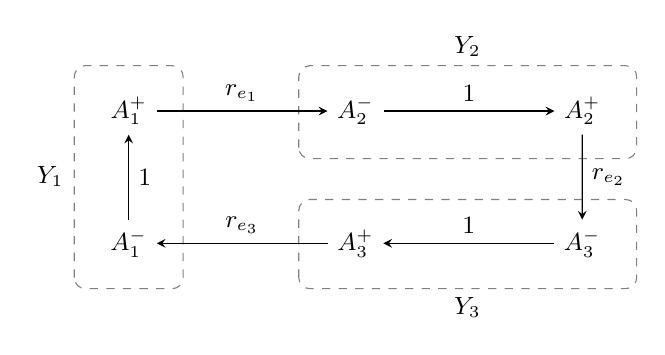
\begin{tikzpicture}[>=stealth,scale=.96,
   every node/.style={font=\small}]
  \draw[dashed,rounded corners,gray] (-.72,-.7) rectangle (.72,2.25);
  \draw[dashed,rounded corners,gray] (2.25,1.02) rectangle (6.72,2.25);
  \draw[dashed,rounded corners,gray] (2.25,-.7) rectangle (6.72,.48);
  \node at (-1.04,.78) {$Y_1$};
  \node at (4.48,2.5) {$Y_2$};
  \node at (4.48,-.95) {$Y_3$};
  \node (a) at (0,1.65) {$A_1^+$};
  \node (b) at (3,1.65) {$A_2^-$};
  \node (c) at (6,1.65) {$A_2^+$};
  \node (d) at (6,-.1) {$A_3^-$};
  \node (e) at (3,-.1) {$A_3^+$};
  \node (f) at (0,-.1) {$A_1^-$};
  \draw[->] (a) -- node[above] {$r_{e_1}$} (b);
  \draw[->] (b) -- node[above] {$1$} (c);
  \draw[->] (c) -- node[right] {$r_{e_2}$} (d);
  \draw[->] (d) -- node[above] {$1$} (e);
  \draw[->] (e) -- node[above] {$r_{e_3}$} (f);
  \draw[->] (f) -- node[right] {$1$} (a);
 \end{tikzpicture}
 \caption{A conductor cycle represented by birational maps between
 minimal strata.  Each dashed box groups two choices inside one dlt
 component; it does not depict geometric intersections.  The arrows
 are birational comparisons, labelled by their pullback multipliers.
 Their composition acts on $A_1^+$ with multiplier
 $r_{e_1}r_{e_2}r_{e_3}$.}
 \label{res:figure}
 \end{figure}

 Choose
 \begin{equation}\label{res:uniform-exponent}
  L=\operatorname{lcm}\{L(q,m):0\le q\le d-1\},
  \qquad a=mL,
 \end{equation}
 where $L(q,m)$ is given by Theorem~\ref{thm:characters}.
 Applying that theorem to \eqref{res:cycle} shows that the product
 of $r_e^L$ around every closed walk is one.  Consequently there
 are constants $c_i\in\C^*$ satisfying
 \begin{equation}\label{res:scales}
  c_i=c_jr_e^L\quad\text{for every oriented edge }e:i\to j.
 \end{equation}
 For completeness, choose a spanning tree in each connected
 component, set $c_i=1$ at one vertex, and determine the other
 constants along its tree paths.  Every additional edge is
 consistent because it closes a walk with product one.  A loop
 imposes precisely $r_e^L=1$, already proved.

 The forms $c_i\theta_i^{\otimes L}$ now have equal residues on
 every pair of conductor branches.  Regard their tuple as a
 rational $a$-canonical form $\sigma$ on $X$: it is an element
 of the product of the degree-$a$ canonical lines of the component
 function fields, a rank-one module over the total quotient ring
 $\prod_i\C(X_i)$.  At every normal
 codimension-one point, its divisor says that it generates the
 line corresponding to $aD$.  At each generic node, its branches
 are generators and have matching residues, so the local rule
 \eqref{res:node-generator} makes it a generator there as well;
 $a$ is even and $B$ avoids those points.

 We explain why this proves Cartierness, rather than only
 triviality after normalization.  Choose a big open immersion
 $j:U\hookrightarrow X$ containing all codimension-one points,
 such that $X$ is Gorenstein on $U$, $aB$ is Cartier on $U$, and
 the preceding local comparisons make $\sigma$ a generator of
 \[
  \mathcal L_{a,U}=\omega_U^{\otimes a}(aB|_U).
 \]
 The divisorial sheaf associated with $aD$ is its $S_2$ extension
 $\mathcal F_a=j_*\mathcal L_{a,U}$.  The generator identifies
 this sheaf with $j_*\OO_U=\OO_X$, the last equality following
 from $S_2$.  Hence $\mathcal F_a$ is invertible.  Equivalently,
 divide $\sigma$ by the $a$th power of a rational canonical
 form, chosen to generate at the generic nodes.  The ratio is
 an invertible element of the total quotient ring whose
 principal divisor is $-aD$ on $U$ and therefore on $X$.
 Thus $aD$ is principal Cartier.  Isolated vertices of the
 conductor graph cause no difficulty: their chosen forms
 already satisfy the required condition.

 Finally let the ground field $k$ be any algebraically closed field
 of characteristic zero.  All the data descend to an algebraically
 closed subfield $k_0\subset k$ of finite transcendence degree over
 $\Q$, including the normalization, conductor, a principal Cartier
 multiple of $D$, and a log resolution of the normalized pair.
 The field $k_0$ embeds in $\C$.  The hypotheses persist under these
 algebraically closed field extensions: $S_2$ and the smooth or
 nodal codimension-one charts are preserved, normalization and
 conductor commute with them, and the coefficients on the chosen
 log resolution test log canonicity after extension.  We therefore
 obtain the degree-$a$ conclusion over $\C$ with the same integer
 \eqref{res:uniform-exponent}.

 On a fixed big Gorenstein open over $k_0$, form $\mathcal F_a$ as
 above.  The open immersion is quasi-compact and separated, since
 $X$ is noetherian.  Flat base change for quasi-coherent sheaves
 therefore shows that this extension by $j_*$ commutes with field
 extension, so its pullback to $\C$ is trivial.  Invertibility
 descends faithfully flatly.  For the resulting line bundle,
 proper cohomology and field extension identify its space of
 global sections after extension with $H^0(X_{\C},\OO_{X_{\C}})
 =\C$.  Its one-dimensional space over $k_0$ therefore has a
 nonzero section whose evaluation becomes an isomorphism over
 $\C$ and hence is already an isomorphism over $k_0$.  Thus
 $\mathcal F_a\simeq\OO$ over $k_0$, and extending to $k$ proves
 the theorem.
\end{proof}

\bibliographystyle{plainnat}
\bibliography{references}
\end{document}
